% !TeX program = xelatex
\documentclass[11pt,a4paper,oneside,openany]{book}

\newcommand{\PrimeraLineaTitulo}{Programar}
\newcommand{\SegundaLineaTitulo}{para resolver}
\newcommand{\TituloLibro}{\PrimeraLineaTitulo\space\SegundaLineaTitulo}
\newcommand{\SubtituloLibro}{Fundamentos del pensamiento computacional y desarrollo de soluciones}
\newcommand{\TipoManuscrito}{Manuscrito académico}
\newcommand{\AutoresLibro}{}
\newcommand{\InstitucionLibro}{}
\newcommand{\AnioEdicion}{2026}

% Tipografía y página
\usepackage{fontspec}
\defaultfontfeatures{Ligatures=TeX}
\setmainfont{lmroman10-regular.otf}[
  BoldFont=lmroman10-bold.otf,
  ItalicFont=lmroman10-italic.otf,
  BoldItalicFont=lmroman10-bolditalic.otf
]
\setsansfont{lmsans10-regular.otf}[
  BoldFont=lmsans10-bold.otf,
  ItalicFont=lmsans10-oblique.otf,
  BoldItalicFont=lmsans10-boldoblique.otf
]
\setmonofont{lmmono10-regular.otf}[
  BoldFont=lmmonolt10-bold.otf,
  ItalicFont=lmmono10-italic.otf,
  Ligatures=NoCommon
]

\usepackage{babel}
\IfFileExists{spanish.ldf}{%
  \babelprovide[main,import=es]{spanish}%
}{%
  \babelprovide[main,import=es]{spanish}%
}
\setlocalecaption{spanish}{contents}{Índice general}
\setlocalecaption{spanish}{listtable}{Índice de tablas}
\setlocalecaption{spanish}{listfigure}{Índice de figuras}
\setlocalecaption{spanish}{table}{Tabla}
\setlocalecaption{spanish}{appendix}{Anexo}

\usepackage{amsmath}
\usepackage{unicode-math}
\setmathfont{latinmodern-math.otf}
\usepackage[left=27mm,right=26mm,top=25mm,bottom=27mm,headheight=15pt]{geometry}
\usepackage[protrusion=true,expansion=false]{microtype}
\usepackage{ragged2e}
\linespread{1.07}
\setlength{\parindent}{0pt}
\setlength{\parskip}{.48em plus .12em minus .08em}
\setlength{\emergencystretch}{1.3em}
\clubpenalty=7500
\widowpenalty=7500
\raggedbottom

% Paleta editorial
\usepackage[table]{xcolor}
\definecolor{Tinta}{HTML}{192C3D}
\definecolor{Azul}{HTML}{173B52}
\definecolor{Verde}{HTML}{086D65}
\definecolor{Gris}{HTML}{466074}
\definecolor{Linea}{HTML}{CAD9DF}
\definecolor{Papel}{HTML}{F2F7F8}
\definecolor{Suave}{HTML}{E4F2EF}

% Jerarquía y encabezados
\usepackage{titlesec}
\usepackage{fancyhdr}
\setcounter{secnumdepth}{1}
\setcounter{tocdepth}{1}
\newcommand{\EtiquetaCapitulo}{%
  \sffamily\bfseries\small\color{Verde}\MakeUppercase{\chaptertitlename}\enspace\thechapter}
\titleformat{\chapter}[display]
  {\sffamily\bfseries\Huge\color{Azul}\RaggedRight}
  {\EtiquetaCapitulo}{.7ex}{}[\vspace{.6ex}{\color{Linea}\titlerule[.65pt]}]
\titleformat{name=\chapter,numberless}[display]
  {\sffamily\bfseries\Huge\color{Azul}\RaggedRight}
  {}{0pt}{}[\vspace{.6ex}{\color{Linea}\titlerule[.65pt]}]
\titlespacing*{\chapter}{0pt}{1.3ex}{2.2ex}
\titleformat{\section}
  {\sffamily\bfseries\Large\color{Azul}\RaggedRight}
  {\textcolor{Verde}{\thesection}}{.7em}{}
\titlespacing*{\section}{0pt}{2.7ex plus .4ex}{.9ex}
\titleformat{\subsection}
  {\sffamily\bfseries\large\color{Azul}\RaggedRight}
  {}{0pt}{}
\titlespacing*{\subsection}{0pt}{1.9ex plus .4ex}{.55ex}

\newcommand{\NotaParte}{}
\titleformat{\part}[display]
  {\sffamily\bfseries\fontsize{38}{43}\selectfont\color{Azul}\RaggedRight}
  {\color{Verde}\normalfont\sffamily\bfseries\large\MakeUppercase{\partname}\enspace\thepart}
  {1.5ex}{}[%
    \par\vspace{.8ex}{\color{Verde}\rule{19mm}{1.1pt}}\par
    \vspace{1.6ex}%
    \normalfont\Large\color{Gris}\NotaParte]
\newcommand{\ParteLibro}[2]{\renewcommand{\NotaParte}{#2}\part{#1}}

\pagestyle{fancy}
\fancyhf{}
\fancyhead[L]{\sffamily\footnotesize\color{Azul}\TituloLibro}
\fancyhead[R]{\sffamily\footnotesize\color{Gris}\nouppercase{\leftmark}}
\fancyfoot[R]{\sffamily\footnotesize\color{Azul}\thepage}
\renewcommand{\headrule}{\vskip-1.5pt\hbox to\headwidth{\color{Linea}\leaders\hrule height.45pt\hfill}}
\renewcommand{\chaptermark}[1]{\markboth{#1}{}}
\fancypagestyle{plain}{%
  \fancyhf{}\fancyfoot[R]{\sffamily\footnotesize\color{Azul}\thepage}%
  \renewcommand{\headrulewidth}{0pt}%
  \renewcommand{\headrule}{}}

\usepackage{enumitem}
\setlist{topsep=.28em,itemsep=.2em,parsep=0pt,partopsep=0pt,leftmargin=1.65em}
\usepackage{needspace}
\usepackage[most]{tcolorbox}
\newtcolorbox{resultados}[1][Resultados de aprendizaje]{
  enhanced, breakable, colback=Suave, colframe=Suave, boxrule=0pt, arc=1.2mm,
  borderline west={1.1pt}{0pt}{Verde}, left=3.6mm, right=3.6mm, top=2.0mm,
  bottom=2.0mm, before skip=.9em, after skip=.9em,
  title={#1}, fonttitle=\sffamily\bfseries\small, coltitle=Verde,
  colbacktitle=Suave, toptitle=2mm, bottomtitle=0mm
}

% Cuadros, figuras, notas y referencias
\usepackage{graphicx}
\usepackage{caption}
\DeclareCaptionFont{rótulo}{\sffamily\bfseries\color{Azul}}
\captionsetup{font=small,labelfont=rótulo,labelsep=period,
  textfont=bf,justification=raggedright,singlelinecheck=false}
\captionsetup[table]{position=above,skip=5pt}
\captionsetup[figure]{position=below,skip=7pt}
\counterwithout{table}{chapter}
\counterwithout{figure}{chapter}
\usepackage{array}
\usepackage{booktabs}
\usepackage{longtable}
\newlength{\AnchoTabla}
\newcolumntype{L}[1]{>{\RaggedRight\arraybackslash}p{#1\AnchoTabla}}
\newcolumntype{R}[1]{>{\raggedleft\arraybackslash}p{#1\AnchoTabla}}
\newcolumntype{C}[1]{>{\centering\arraybackslash}p{#1\AnchoTabla}}
\newenvironment{tablalibro}[2]{%
  \par\needspace{5.3\baselineskip}\begingroup\small
  \setlength{\tabcolsep}{6pt}%
  \setlength{\AnchoTabla}{\dimexpr\linewidth-#1\tabcolsep-#1\tabcolsep+2\tabcolsep\relax}%
  \setlength{\LTleft}{0pt}\setlength{\LTright}{0pt}%
  \setlength{\LTcapwidth}{\linewidth}%
  \setlength{\LTpre}{.55em}\setlength{\LTpost}{.8em}%
  \renewcommand{\arraystretch}{1.24}%
  \arrayrulecolor{Linea}%
  \begin{longtable}{@{}#2@{}}%
}{\end{longtable}\endgroup}
\newcommand{\CabeceraTabla}[1]{\sffamily\bfseries\color{Azul}#1}
\newcommand{\NotaLibro}[1]{{\footnotesize\color{Gris}\textit{Nota.} #1}}
\newcommand{\SigueTabla}[1]{\multicolumn{#1}{@{}l@{}}{\footnotesize\color{Gris}Tabla \thetable\space (continuación)}\\}
\newcommand{\ContinuaTabla}[1]{\multicolumn{#1}{@{}r@{}}{\footnotesize\color{Gris}Continúa en la página siguiente.}\\}
\newcommand{\RefTabla}[1]{\hyperref[#1]{tabla~\ref*{#1}}}
\newcommand{\RefFigura}[1]{\hyperref[#1]{figura~\ref*{#1}}}
\newcommand{\RefCapitulo}[1]{\hyperref[#1]{capítulo~\ref*{#1}}}
\newcommand{\RefAnexo}[1]{\hyperref[#1]{anexo~\ref*{#1}}}

\usepackage{tikz}
\usetikzlibrary{arrows.meta,positioning,shapes.geometric,calc}
\tikzset{
  diagrama nodo/.style={font=\sffamily\small,align=center,inner sep=5pt,
    draw=Linea,fill=Papel,text=Azul,thick,minimum height=8mm},
  diagrama bloque/.style={diagrama nodo,rounded corners=1.3mm},
  diagrama proceso/.style={diagrama nodo},
  diagrama terminal/.style={diagrama nodo,ellipse,fill=Suave,draw=Verde,minimum width=16mm},
  diagrama datos/.style={diagrama nodo,trapezium,
    trapezium left angle=71,trapezium right angle=109,trapezium stretches=true,fill=Suave},
  diagrama decision/.style={diagrama nodo,diamond,aspect=2.45,fill=Suave,draw=Verde,
    inner sep=1.5pt},
  diagrama flecha/.style={-{Latex[length=2.2mm]},draw=Verde,line width=.76pt,rounded corners=1.3pt},
  diagrama union/.style={draw=Gris,line width=.55pt},
  diagrama rama/.style={font=\sffamily\footnotesize,text=Gris,fill=white,inner sep=2pt}
}
\NewDocumentCommand{\FiguraLibro}{m m m m}{%
  \par\addvspace{.8em}%
  \noindent\begin{minipage}{\linewidth}
    \centering
    \input{figuras/#1}\par
    \captionof{figure}{#2}\label{#3}%
    \if\relax\detokenize{#4}\relax\else
      \RaggedRight\NotaLibro{#4}\par
    \fi
  \end{minipage}\par\addvspace{.8em}%
}

% Listados de texto plano y código incluidos desde los archivos ejecutables.
\usepackage{listings}
\lstdefinestyle{libro}{
  basicstyle=\small\ttfamily\color{Tinta}, backgroundcolor=\color{Papel},
  frame=leftline, framerule=1pt, rulecolor=\color{Linea}, framesep=5pt,
  xleftmargin=2mm, xrightmargin=.75mm, aboveskip=.7em, belowskip=.65em,
  columns=fullflexible, keepspaces=true, upquote=true, tabsize=4,
  showstringspaces=false, breaklines=true, breakatwhitespace=false,
  keywordstyle=\color{Verde}\bfseries, commentstyle=\color{Gris}\itshape,
  stringstyle=\color{Azul},
  literate=
    {á}{{á}}1 {é}{{é}}1 {í}{{í}}1 {ó}{{ó}}1 {ú}{{ú}}1
    {Á}{{Á}}1 {É}{{É}}1 {Í}{{Í}}1 {Ó}{{Ó}}1 {Ú}{{Ú}}1
    {ñ}{{ñ}}1 {Ñ}{{Ñ}}1 {ü}{{ü}}1 {²}{{²}}1 {←}{{$\leftarrow$}}1
}
\NewDocumentCommand{\Python}{O{} m}{\lstinputlisting[style=libro,language=Python,#1]{recursos/#2}}
\NewDocumentCommand{\Pseudocodigo}{m}{\lstinputlisting[style=libro]{recursos/pseudocodigo/#1}}
\NewDocumentCommand{\Salida}{m}{\lstinputlisting[style=libro]{recursos/salidas/#1}}
\newcommand{\Codigo}[1]{\texttt{#1}}

\newcommand{\CapituloFinal}[1]{%
  \chapter*{#1}\markboth{#1}{}\addcontentsline{toc}{chapter}{#1}}
\newcommand{\SeccionLibro}[2][]{%
  \section*{#2}%
  \if\relax\detokenize{#1}\relax
    \addcontentsline{toc}{section}{#2}%
  \else
    \addcontentsline{toc}{section}{#1}%
  \fi
}
\newcounter{ejemplo}[chapter]
\renewcommand{\theejemplo}{\thechapter.\arabic{ejemplo}}
\newcommand{\Ejemplo}[1]{%
  \refstepcounter{ejemplo}\subsection*{Ejemplo \theejemplo. #1}}

\usepackage[authoryear,round]{natbib}
\setlength{\bibhang}{1.5em}
\setlength{\bibsep}{.45em}
\renewcommand{\bibsection}{\CapituloFinal{Referencias bibliográficas}}
\usepackage[unicode,bookmarksnumbered,bookmarksopen,
  colorlinks,linkcolor=Azul,citecolor=Verde,urlcolor=Verde]{hyperref}
\usepackage{bookmark}
\hypersetup{
  pdftitle={\TituloLibro. \SubtituloLibro},
  pdfsubject={\TipoManuscrito},
  pdflang={es-PE}
}
\AtBeginDocument{\color{Tinta}}


\begin{document}

\frontmatter
\begin{titlepage}
  \thispagestyle{empty}
  \begin{tikzpicture}[remember picture,overlay]
    \fill[Papel] (current page.south west) rectangle (current page.north east);
    \fill[Azul] (current page.north west)
      rectangle ([yshift=-135mm]current page.north east);
    \fill[Verde] ([yshift=-135mm]current page.north west)
      rectangle ([yshift=-136mm]current page.north east);
    \begin{scope}[shift={([xshift=105mm,yshift=87mm]current page.south west)}]
      \node[inner sep=0pt,opacity=.27] at (2.95,1.4)
        {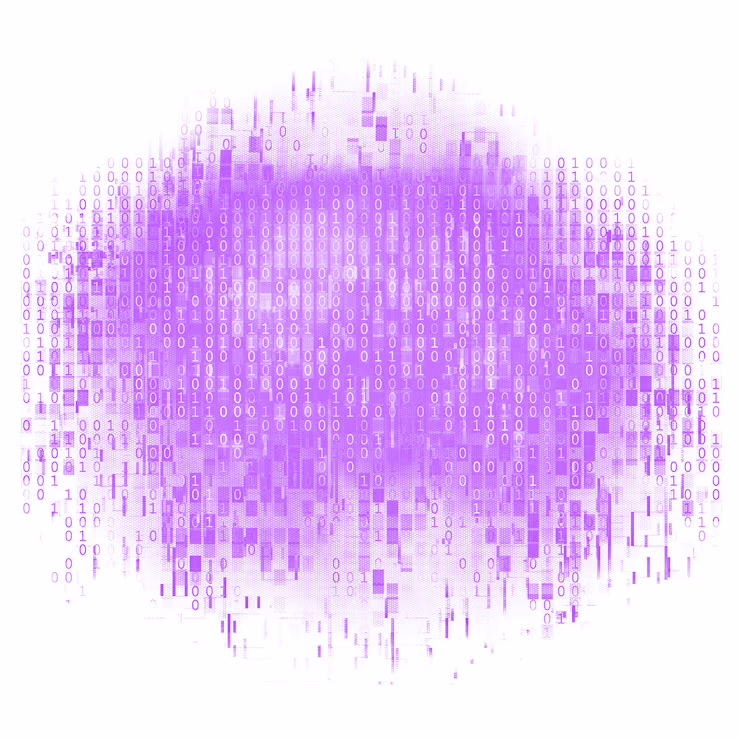
\includegraphics[width=99mm]{figuras/portada-codigo.png}};
      \node[inner sep=0pt] at (-.15,0)
        {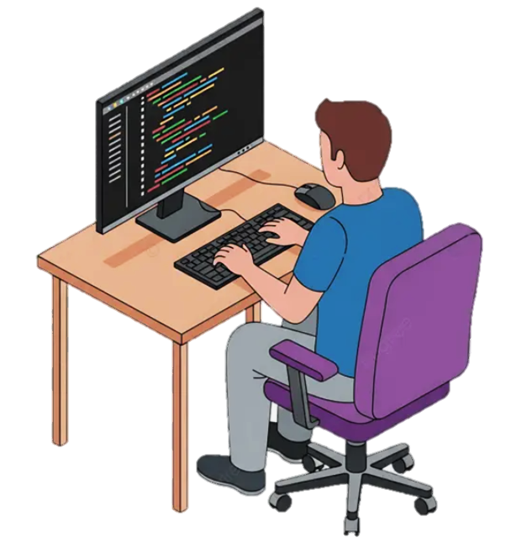
\includegraphics[height=101mm]{figuras/portada-programacion.png}};
    \end{scope}
    \node[anchor=north west,inner sep=0pt,text=white,text width=158mm]
      at ([xshift=26mm,yshift=-23mm]current page.north west) {%
        \sffamily\bfseries\normalsize\InstitucionLibro\par
        \vspace{9mm}
        {\fontsize{48}{50}\selectfont\spaceskip=.28em
          \PrimeraLineaTitulo\par\SegundaLineaTitulo\par}
        \vspace{5mm}
        {\mdseries\fontsize{16}{21}\selectfont
          \PrimeraLineaSubtitulo\par\SegundaLineaSubtitulo\par}
      };
    \draw[white!35!Azul,line width=.45pt]
      ([xshift=26mm,yshift=-99mm]current page.north west)
      -- ([xshift=-26mm,yshift=-99mm]current page.north east);
    \node[anchor=north west,inner sep=0pt,text=white,font=\sffamily\normalsize]
      at ([xshift=26mm,yshift=-105mm]current page.north west) {%
        \begin{tabular*}{158mm}{@{}p{75mm}@{\extracolsep{\fill}}p{75mm}@{}}
          \PrimerAutor & \SegundoAutor\\[.9mm]
          \TercerAutor & \CuartoAutor\\[.9mm]
          \QuintoAutor & \SextoAutor
        \end{tabular*}
      };
    \draw[Linea,line width=.55pt] ([xshift=26mm,yshift=29mm]current page.south west)
      -- ([xshift=-26mm,yshift=29mm]current page.south east);
    \node[anchor=east,inner sep=0pt,text=Azul,font=\sffamily\bfseries\normalsize]
      at ([xshift=-26mm,yshift=20mm]current page.south east) {\AnioEdicion};
  \end{tikzpicture}
  \null\vfill
\end{titlepage}
\setcounter{page}{2}

\tableofcontents
\chapter{Introducción}

La resolución de problemas es una actividad inherente al ser humano. Desde las decisiones más sencillas de la vida cotidiana hasta el desarrollo de complejos sistemas tecnológicos, las personas necesitan identificar dificultades, analizar alternativas y establecer procedimientos que permitan alcanzar determinados objetivos.

La incorporación de las computadoras en diferentes ámbitos de la sociedad ha ampliado considerablemente las posibilidades de resolver problemas. Sin embargo, una computadora no determina por sí misma qué problema debe solucionar ni qué resultado se considera satisfactorio. Es necesario formular el problema, establecer sus condiciones y desarrollar procedimientos que puedan ser representados y ejecutados computacionalmente.

\citet{farrell2013} aborda la importancia de desarrollar la lógica de los programas antes de proceder a su implementación mediante un lenguaje de programación. Desde esta perspectiva, el diseño de una solución constituye una etapa fundamental para obtener programas organizados y funcionales.

Por ejemplo, si una institución educativa necesita determinar la condición académica de sus estudiantes a partir de sus calificaciones, el proceso no comienza necesariamente escribiendo código. Primero es necesario identificar qué información se requiere, cómo se calcularán los resultados, cuáles son las condiciones de aprobación y qué información deberá proporcionar el sistema.

Este procedimiento aplica estrategias del pensamiento computacional como la descomposición, el reconocimiento de patrones, la abstracción, la generalización y el diseño de algoritmos. Estas habilidades sirven en informática, educación, ingeniería, administración y medicina. La \RefFigura{fig:proceso-resolucion} muestra las etapas del proceso.

\FiguraLibro{01-proceso-resolucion}{Proceso general de resolución de problemas computacionales}{fig:proceso-resolucion}{Elaboración propia.}

El libro utiliza la programación para construir y evaluar soluciones. Los ejemplos emplean Python por su sintaxis accesible. Los principios pueden aplicarse en otros lenguajes.

\listoftables
\listoffigures

\mainmatter
\ParteLibro{Comprensión de problemas y diseño de soluciones}
  {Del análisis de situaciones cotidianas a algoritmos que pueden comprobarse antes de programar.}

\chapter{Fundamentos del pensamiento computacional y análisis de problemas}
\label{cap:01-pensamiento-computacional}
\chaptermark{Pensamiento computacional}

La capacidad de resolver problemas representa uno de los pilares fundamentales de las ciencias de la computación. Antes de construir un programa informático, es necesario comprender la situación que se desea solucionar, identificar sus componentes y establecer una estrategia que permita alcanzar los resultados esperados.

Este capítulo introduce los fundamentos del pensamiento computacional como una metodología de razonamiento aplicable a diferentes situaciones de la vida cotidiana y del ámbito profesional.

\begin{resultados}
  \begin{itemize}
    \item Distinguir una necesidad cotidiana de un problema formulado para una computadora.
    \item Aplicar descomposición, reconocimiento de patrones, abstracción y generalización.
    \item Especificar objetivos, entradas, procesos, salidas y criterios de aceptación.
  \end{itemize}
\end{resultados}

\section{La resolución de problemas en la vida cotidiana}

Las personas se enfrentan constantemente a situaciones que requieren tomar decisiones y encontrar soluciones. Organizar un horario de estudios, administrar un presupuesto familiar, seleccionar una ruta de transporte o distribuir las actividades de un proyecto son ejemplos de problemas que requieren razonamiento y planificación.

Aunque estas actividades no siempre involucran el uso de computadoras, poseen características que permiten estudiarlas desde una perspectiva computacional.

\subsection{Concepto de problema}

Un problema puede definirse como una situación en la que existe una diferencia entre un estado actual y un estado deseado, cuya transformación requiere la aplicación de determinadas acciones o procedimientos. La \RefFigura{fig:elementos-problema} representa esta transición.

\FiguraLibro{02-elementos-problema}{Elementos generales de un problema}{fig:elementos-problema}{Elaboración propia.}

Desde esta perspectiva, resolver un problema implica identificar la situación inicial, establecer el objetivo y determinar las acciones necesarias para alcanzarlo.

\Needspace{11\baselineskip}
\subsection{Elementos de un problema}

\begin{tablalibro}{2}{L{0.28}L{0.72}}
\caption{Elementos de un problema}\label{tab:elementos-de-un-problema}\\
\toprule
\rowcolor{Papel}
\CabeceraTabla{Elemento} & \CabeceraTabla{Descripción} \\
\midrule
\endfirsthead
\SigueTabla{2}
\toprule
\rowcolor{Papel}
\CabeceraTabla{Elemento} & \CabeceraTabla{Descripción} \\
\midrule
\endhead
\midrule
\ContinuaTabla{2}
\endfoot
\bottomrule
\endlastfoot

Estado inicial & Situación en la que se encuentra el problema. \\
Objetivo & Resultado que se desea alcanzar. \\
Datos disponibles & Información necesaria para formular una solución. \\
Restricciones & Condiciones que deben respetarse. \\
Estrategia & Procedimientos seleccionados para resolver el problema. \\
Resultado & Producto obtenido después de aplicar la solución. \\
\end{tablalibro}


\subsection{Ejemplo práctico: administración de un presupuesto semanal}

Un estudiante dispone de S/ 100 para cubrir sus gastos semanales. Durante la semana necesita destinar dinero a transporte, alimentación y materiales educativos. Su objetivo es determinar cuánto dinero le quedará disponible después de cubrir dichos gastos. La \RefTabla{tab:presupuesto-semanal} reúne los importes del ejemplo.

\begin{tablalibro}{2}{L{0.69}R{0.31}}
\caption{Presupuesto semanal}\label{tab:presupuesto-semanal}\\
\toprule
\rowcolor{Papel}
\CabeceraTabla{Concepto} & \CabeceraTabla{Importe} \\
\midrule
\endfirsthead
\SigueTabla{2}
\toprule
\rowcolor{Papel}
\CabeceraTabla{Concepto} & \CabeceraTabla{Importe} \\
\midrule
\endhead
\midrule
\endfoot
\bottomrule
\endlastfoot

Presupuesto inicial & S/ 100 \\
Transporte & S/ 25 \\
Alimentación & S/ 40 \\
Materiales educativos & S/ 15 \\
\textbf{Total de gastos} & \textbf{S/ 80} \\
\textbf{Saldo disponible} & \textbf{S/ 20} \\
\end{tablalibro}


La solución consiste en identificar los gastos, calcular su suma y restar el resultado del presupuesto inicial.

El saldo se obtiene con la siguiente expresión.

\[ S = P - (T + A + M) \]

Las variables representan el saldo, el presupuesto inicial y los tres gastos.

\begin{itemize}
\item \(S\): saldo disponible.
\item \(P\): presupuesto inicial.
\item \(T\): gasto de transporte.
\item \(A\): gasto de alimentación.
\item \(M\): gasto de materiales.
\end{itemize}

Este ejemplo demuestra que una situación cotidiana puede transformarse en una solución organizada y expresarse mediante operaciones matemáticas. Posteriormente, este mismo procedimiento podrá representarse mediante un algoritmo e implementarse utilizando un lenguaje de programación.

\subsection{Etapas de la resolución de problemas}

\FiguraLibro{03-etapas-resolucion}{Etapas de la resolución de problemas}{fig:etapas-resolucion}{Elaboración propia.}

La aplicación sistemática de estas etapas facilita el desarrollo de soluciones organizadas. Cuando los resultados obtenidos no coinciden con los objetivos establecidos, es necesario revisar las decisiones adoptadas, identificar posibles errores y modificar la estrategia.

Por consiguiente, la resolución de problemas debe comprenderse como un proceso que puede requerir múltiples intentos, evaluaciones y mejoras.

\section{Problemas que pueden resolverse mediante computadoras}

No todos los problemas de la vida cotidiana requieren una computadora para ser resueltos. Sin embargo, cuando una situación involucra operaciones repetitivas, grandes cantidades de información o decisiones que pueden expresarse mediante condiciones precisas, el uso de un sistema computacional puede facilitar considerablemente su solución. Para determinar si resulta conveniente emplear una computadora, es necesario examinar la naturaleza del problema y la posibilidad de representar sus datos y procedimientos de manera formal.

\textcite[pp.~4–6]{farrell2013} explica que la ejecución de un programa implica realizar instrucciones y que, habitualmente, estas permiten recibir datos, procesarlos y producir resultados. También distingue los errores de sintaxis de los errores lógicos: un programa puede ejecutarse sin que su resultado sea correcto. Esta distinción permite comprender que la capacidad de procesamiento de una computadora no reemplaza el análisis previo del problema ni el diseño cuidadoso de la solución.

\subsection{Características de los problemas computacionales}

Un problema computacional es una situación que puede formularse de manera que una computadora ejecute un procedimiento para obtener una respuesta, generar un resultado o contribuir a una decisión. Para los problemas introductorios que se estudian en este libro, conviene reconocer las siguientes características:

\begin{itemize}
\item Objetivo definido. Se puede establecer qué resultado se espera obtener.
\item Datos representables. La información necesaria puede expresarse mediante números, textos, valores lógicos u otras representaciones digitales.
\item Reglas identificables. Es posible especificar operaciones, condiciones o criterios para transformar los datos.
\item Procedimiento ejecutable. Las operaciones pueden traducirse en instrucciones que una computadora sea capaz de realizar.
\item Resultado evaluable. Se dispone de criterios para comprobar si la respuesta obtenida satisface el objetivo.
\end{itemize}

Estas características constituyen una guía práctica de análisis, no una definición matemática exhaustiva de la computabilidad. Un problema puede admitir una formulación computacional y, aun así, resultar demasiado costoso de resolver exactamente con los recursos disponibles. En otros casos, la dificultad consiste en precisar los criterios o conseguir datos adecuados.

\subsection{Tipos de problemas que admiten soluciones computacionales}

Los problemas pueden clasificarse de acuerdo con la operación predominante que requiere su solución. La siguiente tabla presenta una clasificación didáctica con ejemplos de diferentes ámbitos. Las categorías no son excluyentes: una misma aplicación puede combinar varias de ellas.

\begin{tablalibro}{2}{L{0.31}L{0.69}}
\caption{Clasificación de problemas computacionales según su finalidad}\label{tab:clasificacion-de-problemas-computacionales-segun-su-finalidad}\\
\toprule
\rowcolor{Papel}
\CabeceraTabla{Tipo de problema} & \CabeceraTabla{Ejemplo de aplicación} \\
\midrule
\endfirsthead
\SigueTabla{2}
\toprule
\rowcolor{Papel}
\CabeceraTabla{Tipo de problema} & \CabeceraTabla{Ejemplo de aplicación} \\
\midrule
\endhead
\midrule
\ContinuaTabla{2}
\endfoot
\bottomrule
\multicolumn{2}{@{}p{\linewidth}@{}}{\NotaLibro{Clasificación y ejemplos de elaboración propia.}}\\
\endlastfoot

Cálculo numérico & Determinar el importe de una compra a partir de los precios y las cantidades. \\
Búsqueda y recuperación & Localizar el registro de un estudiante mediante su código. \\
Ordenamiento & Organizar productos de menor a mayor precio. \\
Clasificación y decisión & Determinar si una calificación cumple una condición de aprobación. \\
Automatización de tareas & Generar reportes periódicos a partir de registros de ventas. \\
Optimización & Seleccionar una distribución de recursos que reduzca costos bajo ciertas restricciones. \\
\end{tablalibro}


\subsection{Ejemplo práctico: control de existencias en una tienda}

Una tienda necesita identificar los productos que deben reponerse. El encargado revisa diariamente las cantidades disponibles y las compara con un nivel mínimo establecido para cada producto. Cuando la cantidad disponible es inferior al mínimo, el producto debe incorporarse a una lista de reposición.

En lugar de efectuar manualmente esta comparación para todos los productos, se propone una solución computacional que reciba los registros de existencias, compare cada cantidad con su mínimo y genere un listado con los productos que requieren atención.

Entrada: Código del producto, cantidad disponible y cantidad mínima.

Procesamiento: Comparar la cantidad disponible con la cantidad mínima de cada producto.

Salida: Listado de productos cuya cantidad disponible es inferior al mínimo.

\begin{tablalibro}{4}{L{0.39}R{0.19}R{0.17}C{0.25}}
\caption{Datos de prueba para el control de existencias}\label{tab:datos-de-prueba-para-el-control-de-existencias}\\
\toprule
\rowcolor{Papel}
\CabeceraTabla{Producto} & \CabeceraTabla{Disponible} & \CabeceraTabla{Mínimo} & \CabeceraTabla{¿Reponer?} \\
\midrule
\endfirsthead
\SigueTabla{4}
\toprule
\rowcolor{Papel}
\CabeceraTabla{Producto} & \CabeceraTabla{Disponible} & \CabeceraTabla{Mínimo} & \CabeceraTabla{¿Reponer?} \\
\midrule
\endhead
\midrule
\endfoot
\bottomrule
\endlastfoot

Cuadernos & 12 & 20 & Sí \\
Lápices & 35 & 15 & No \\
Borradores & 10 & 10 & No \\
Reglas & 4 & 8 & Sí \\
\end{tablalibro}


El resultado esperado es una lista que contiene cuadernos y reglas. Obsérvese que los borradores no se incluyen, porque la regla establecida exige que la cantidad disponible sea estrictamente inferior al mínimo. Si el encargado quisiera reponer también los productos que tienen exactamente la cantidad mínima, sería necesario modificar la condición. Esta diferencia muestra cómo una pequeña variación en la formulación del problema puede cambiar los resultados del programa.

\subsection{Alcances y limitaciones de las soluciones computacionales}

Una computadora puede ejecutar operaciones con rapidez, almacenar información y aplicar criterios de manera consistente. No obstante, un sistema basado en reglas depende de la calidad de sus datos y de la corrección de los procedimientos definidos. Por ejemplo, si el inventario registra una cantidad equivocada, la lista de reposición podría ser incorrecta aunque el programa realice correctamente todas las comparaciones.

Asimismo, existen situaciones en las que no basta con aplicar reglas explícitas. La identificación de objetos en imágenes, por ejemplo, puede requerir modelos que aprendan a partir de datos. Sus resultados no necesariamente son exactos y deben evaluarse antes de emplearlos en decisiones relevantes. Este ejemplo permite distinguir los procedimientos deterministas sencillos, que serán el centro de los primeros capítulos, de otras estrategias computacionales más avanzadas.

Por tanto, antes de decidir que una computadora debe resolver un problema, conviene preguntarse si el objetivo está suficientemente definido, si los datos están disponibles, si el procedimiento es viable y cómo se verificará el resultado. Estas preguntas preparan al estudiante para comprender el pensamiento computacional, tema del siguiente apartado.

\section{Concepto e importancia del pensamiento computacional}

El pensamiento computacional emplea conceptos de la informática para formular problemas y organizar soluciones. \textcite{wing2006} destaca dos recursos para tratar tareas complejas: descomponerlas y elegir una representación que conserve lo relevante. Este capítulo combina esas prácticas con el reconocimiento de patrones y la generalización. La selección de estrategias depende de qué se necesita resolver y cómo se puede comprobar el resultado.

La planificación de la lógica constituye una etapa anterior a la codificación. \textcite[pp.~8–10]{farrell2013} explica que el desarrollo de programas exige comprender las necesidades del usuario, determinar el resultado esperado y organizar las operaciones que conducen a dicho resultado. Esta perspectiva ofrece un punto de partida para relacionar el pensamiento computacional con la práctica de la programación.

\subsection{Componentes del pensamiento computacional}

Para los fines didácticos de este libro, se distinguen cinco estrategias complementarias. No representan una secuencia rígida: durante el análisis es frecuente regresar a una estrategia anterior cuando aparece información nueva o se descubre una condición que no había sido considerada.

\begin{tablalibro}{3}{L{0.28}L{0.34}L{0.38}}
\caption{Estrategias del pensamiento computacional}\label{tab:estrategias-del-pensamiento-computacional}\\
\toprule
\rowcolor{Papel}
\CabeceraTabla{Estrategia} & \CabeceraTabla{Pregunta orientadora} & \CabeceraTabla{Ejemplo} \\
\midrule
\endfirsthead
\SigueTabla{3}
\toprule
\rowcolor{Papel}
\CabeceraTabla{Estrategia} & \CabeceraTabla{Pregunta orientadora} & \CabeceraTabla{Ejemplo} \\
\midrule
\endhead
\midrule
\endfoot
\bottomrule
\multicolumn{3}{@{}p{\linewidth}@{}}{\NotaLibro{Elaboración propia.}}\\
\endlastfoot

Descomposición & ¿En qué partes puedo dividir el problema? & Separar registro, cálculo y reporte de notas. \\
Reconocimiento de patrones & ¿Qué se repite o se parece? & Identificar cálculos iguales en distintos cursos. \\
Abstracción & ¿Qué información necesito conservar? & Considerar las calificaciones y sus pesos. \\
Generalización & ¿Cómo reutilizar la solución? & Aplicar el cálculo a distintos estudiantes. \\
Diseño algorítmico & ¿Qué pasos permiten obtener el resultado? & Validar datos, calcular y comunicar el promedio. \\
\end{tablalibro}


\subsection{Importancia en la formación académica y profesional}

El pensamiento computacional ayuda a organizar problemas complejos, explicar decisiones y establecer criterios de comprobación. En el ámbito educativo permite estructurar investigaciones, analizar información y construir modelos sencillos. En ingeniería facilita la especificación de procesos y la identificación de restricciones. En administración contribuye a organizar tareas repetitivas y a detectar inconsistencias en registros.

Su utilidad no implica que todo problema deba automatizarse. Una solución puede ser técnicamente posible y, aun así, resultar inadecuada por su costo, por la falta de datos confiables o por sus consecuencias para las personas. El análisis debe considerar tanto la viabilidad técnica como las necesidades de quienes utilizarán el resultado.

\subsection{Ejemplo: organización de una jornada de estudio}

Un estudiante dispone de 180 minutos para preparar tres asignaturas. Decide reservar 15 minutos de descanso y distribuir los 165 minutos restantes según la dificultad de cada asignatura. Si establece pesos de 3, 2 y 1, puede asignar 82,5; 55 y 27,5 minutos, respectivamente. La solución identifica recursos, restricciones y una regla de distribución. Si el tiempo disponible cambia, la misma regla puede aplicarse con nuevos datos.

Antes de automatizar esta distribución, conviene verificar que los pesos sean positivos, que el descanso no exceda el tiempo total y que el reparto sea compatible con las necesidades reales del estudiante. El ejemplo muestra que razonar computacionalmente incluye formular condiciones y revisar resultados, además de efectuar cálculos.

\section{Descomposición de problemas en partes más pequeñas}

La descomposición consiste en dividir un problema complejo en subproblemas cuya comprensión y tratamiento resulten más manejables. Cada parte debe tener una finalidad identificable y contribuir al objetivo general. Esta estrategia reduce la cantidad de detalles que deben considerarse simultáneamente y facilita localizar las dificultades que requieren mayor atención.

En el diseño de programas, \textcite[pp.~48–50]{farrell2013} relaciona la división de tareas con la modularización, la abstracción y la reutilización. Aunque en este capítulo todavía no se implementan módulos de código, la descomposición permite preparar una estructura que más adelante podrá traducirse en componentes de un programa.

\subsection{Procedimiento de descomposición}

\begin{itemize}
\item Precisar el objetivo general y delimitar qué queda fuera del problema.
\item Identificar las tareas principales y el resultado de cada una.
\item Dividir las tareas complejas hasta obtener actividades comprensibles.
\item Establecer las dependencias entre las partes y la información que intercambian.
\item Revisar que la integración de las partes satisfaga el objetivo original.
\end{itemize}

\subsection{Ejemplo: sistema de préstamo de libros}

Una biblioteca escolar necesita registrar préstamos y devoluciones. Intentar resolver todas las operaciones como una sola tarea dificulta identificar las reglas. Es preferible distinguir la identificación del lector, la consulta de disponibilidad, el registro del préstamo y la actualización de la devolución.

\begin{tablalibro}{3}{L{0.28}L{0.34}L{0.38}}
\caption{Descomposición de un sistema de préstamos}\label{tab:descomposicion-de-un-sistema-de-prestamos}\\
\toprule
\rowcolor{Papel}
\CabeceraTabla{Subproblema} & \CabeceraTabla{Información requerida} & \CabeceraTabla{Resultado} \\
\midrule
\endfirsthead
\SigueTabla{3}
\toprule
\rowcolor{Papel}
\CabeceraTabla{Subproblema} & \CabeceraTabla{Información requerida} & \CabeceraTabla{Resultado} \\
\midrule
\endhead
\midrule
\endfoot
\bottomrule
\multicolumn{3}{@{}p{\linewidth}@{}}{\NotaLibro{Elaboración propia.}}\\
\endlastfoot

Identificar lector & Código del lector & Lector reconocido o aviso de error \\
Consultar ejemplar & Código del ejemplar & Disponibilidad confirmada \\
Registrar préstamo & Lector, ejemplar y fecha & Préstamo registrado \\
Registrar devolución & Identificador del préstamo & Préstamo cerrado y ejemplar disponible \\
\end{tablalibro}


Las partes no son necesariamente independientes. El registro del préstamo requiere que el lector esté identificado y que el ejemplar se encuentre disponible. Si una consulta falla, no se debe modificar el estado del ejemplar. Definir estas dependencias evita que cada componente funcione correctamente por separado, pero produzca un resultado incorrecto al integrarse.

\subsection{Criterios de una buena descomposición}

Una división adecuada asigna a cada parte una responsabilidad clara, evita duplicar tareas y permite verificar resultados parciales. Una división demasiado extensa puede ocultar dificultades; una información excesivamente detallada puede generar complejidad innecesaria. El nivel de detalle debe corresponder al propósito del análisis y a la experiencia de quienes participan en él.

\section{Reconocimiento de patrones y semejanzas}

El reconocimiento de patrones consiste en identificar regularidades, relaciones o estructuras semejantes entre situaciones. En la resolución de problemas, permite aprovechar conocimientos previos y evitar diseñar desde el inicio procedimientos que ya se han aplicado con éxito en circunstancias equivalentes.

Un patrón no siempre es una repetición exacta. Dos problemas pueden utilizar datos diferentes y compartir una misma estructura lógica. Por ejemplo, calcular el total de una compra y calcular el costo de materiales de un proyecto requieren multiplicar cantidades por precios unitarios y sumar los importes obtenidos.

\Needspace{11\baselineskip}
\subsection{Patrones frecuentes en problemas computacionales}

\begin{tablalibro}{3}{L{0.28}L{0.34}L{0.38}}
\caption{Patrones de resolución y ejemplos}\label{tab:patrones-de-resolucion-y-ejemplos}\\
\toprule
\rowcolor{Papel}
\CabeceraTabla{Patrón} & \CabeceraTabla{Operación común} & \CabeceraTabla{Aplicación} \\
\midrule
\endfirsthead
\SigueTabla{3}
\toprule
\rowcolor{Papel}
\CabeceraTabla{Patrón} & \CabeceraTabla{Operación común} & \CabeceraTabla{Aplicación} \\
\midrule
\endhead
\midrule
\endfoot
\bottomrule
\endlastfoot

Acumulación & Sumar valores sucesivos & Total de gastos \\
Conteo & Incrementar un contador & Número de asistentes \\
Comparación & Evaluar una condición & Productos bajo el mínimo \\
Búsqueda & Localizar un elemento & Encontrar un código de matrícula \\
Clasificación & Asignar una categoría & Agrupar solicitudes por estado \\
\end{tablalibro}


\subsection{Ejemplo: análisis de asistencia}

Un docente registra cinco sesiones con los estados presente, ausente, presente, presente y ausente. Para obtener la cantidad de asistencias, se reconoce una operación que debe repetirse para cada registro: examinar el estado e incrementar el conteo cuando corresponda. El resultado es tres asistencias de cinco sesiones, equivalente al 60 \% si todas las sesiones tienen el mismo valor.

La misma estructura permite contar entregas de tareas o productos defectuosos, siempre que se cambie el criterio de selección. Sin embargo, si una sesión justificada debe excluirse del denominador, la regla de cálculo ya no es idéntica. Reconocer semejanzas exige también identificar diferencias que afectan la solución.

\subsection{Patrones y evidencia}

En problemas basados en datos, una regularidad observada puede orientar una hipótesis, pero no demuestra que se mantenga en todos los casos ni establece una relación causal. Por ello, los patrones deben contrastarse con ejemplos nuevos, excepciones y datos que no se utilizaron para formular la regla. Esta precaución será especialmente relevante en aplicaciones de aprendizaje automático.

\section{Abstracción e identificación de información relevante}

La abstracción permite representar un problema conservando las características que son necesarias para alcanzar un objetivo y dejando de lado detalles que no afectan la solución. \textcite[p.~49]{farrell2013} presenta la abstracción como un recurso que facilita comprender tareas complejas al concentrarse en sus propiedades esenciales.

La relevancia de un dato depende del propósito. Un dato puede ser indispensable en una aplicación y prescindible en otra. Por tanto, abstraer no significa eliminar información arbitrariamente, sino justificar qué datos se conservan, qué relaciones se representan y qué detalles se omiten.

\subsection{Ejemplo: cálculo de una tarifa de transporte}

Supóngase una tarifa didáctica compuesta por S/ 4 de cargo fijo y S/ 1,50 por kilómetro recorrido. Para calcular el importe se necesita la distancia y los valores de la tarifa. El color del vehículo o el nombre del conductor no intervienen en el cálculo. En cambio, si se incorporan recargos nocturnos, la hora del viaje pasa a ser relevante.

\begin{tablalibro}{3}{L{0.28}C{0.18}L{0.54}}
\caption{Selección de información para calcular una tarifa}\label{tab:seleccion-de-informacion-para-calcular-una-tarifa}\\
\toprule
\rowcolor{Papel}
\CabeceraTabla{Dato} & \CabeceraTabla{¿Relevante?} & \CabeceraTabla{Justificación} \\
\midrule
\endfirsthead
\SigueTabla{3}
\toprule
\rowcolor{Papel}
\CabeceraTabla{Dato} & \CabeceraTabla{¿Relevante?} & \CabeceraTabla{Justificación} \\
\midrule
\endhead
\midrule
\endfoot
\bottomrule
\endlastfoot

Distancia recorrida & Sí & Determina el cargo variable. \\
Cargo fijo & Sí & Forma parte del importe. \\
Precio por kilómetro & Sí & Determina el costo por distancia. \\
Color del vehículo & No & No modifica la tarifa definida. \\
Hora del viaje & Depende & Es necesaria si existen recargos horarios. \\
\end{tablalibro}


Con una distancia de 6 km, el importe del ejemplo es S/ 4 + S/ 1,50 × 6 = S/ 13. Esta representación supone que no existen peajes, descuentos ni otras condiciones. Si tales condiciones forman parte del problema real, deberán añadirse al modelo antes de utilizarlo.

\subsection{Niveles de abstracción}

En un nivel conceptual se describen objetivos y entidades; en un nivel lógico se identifican datos, relaciones y reglas; en un nivel de implementación se establecen instrucciones y estructuras concretas. En el presente capítulo se trabaja principalmente en los dos primeros niveles. Esta separación permite discutir el problema sin depender todavía de la sintaxis de un lenguaje.

Una abstracción insuficiente conserva detalles que dificultan comprender el problema. Una abstracción excesiva elimina condiciones necesarias y puede generar resultados incorrectos. Para evaluar una representación, debe comprobarse si permite responder las preguntas planteadas sin introducir supuestos injustificados.

\section{Generalización de soluciones para diferentes situaciones}

La generalización consiste en transformar una solución particular en un procedimiento aplicable a una familia de problemas que comparten características esenciales. Se apoya en el reconocimiento de patrones y en la abstracción: primero se identifica aquello que permanece constante y después se expresa como una regla que admite diferentes valores de entrada.

\subsection{De una solución particular a una regla general}

Considérese una compra de tres cuadernos a S/ 5 cada uno. El importe es S/ 15. Si se desea resolver compras de otros productos, no conviene conservar los valores 3 y 5 como parte fija del procedimiento. Se sustituyen por datos variables: cantidad y precio unitario. Así, el importe se obtiene multiplicando ambos valores.

Para una compra con varios productos, la regla se amplía: calcular el importe de cada producto y sumar los importes. El número de productos deja de estar fijado de antemano. El procedimiento puede utilizarse para una compra de uno, dos o más artículos, bajo las mismas condiciones de cálculo.

\begin{tablalibro}{4}{L{0.43}R{0.16}R{0.21}R{0.20}}
\caption{Aplicación de una regla general de cálculo}\label{tab:aplicacion-de-una-regla-general-de-calculo}\\
\toprule
\rowcolor{Papel}
\CabeceraTabla{Situación} & \CabeceraTabla{Cantidad} & \CabeceraTabla{Precio unitario} & \CabeceraTabla{Importe} \\
\midrule
\endfirsthead
\SigueTabla{4}
\toprule
\rowcolor{Papel}
\CabeceraTabla{Situación} & \CabeceraTabla{Cantidad} & \CabeceraTabla{Precio unitario} & \CabeceraTabla{Importe} \\
\midrule
\endhead
\midrule
\endfoot
\bottomrule
\endlastfoot

Cuadernos & 3 & S/ 5 & S/ 15 \\
Lápices & 8 & S/ 1,50 & S/ 12 \\
Carpetas & 2 & S/ 9 & S/ 18 \\
\end{tablalibro}


\subsection{Condiciones y límites de la generalización}

Generalizar no significa que una solución sea válida para cualquier problema. La regla anterior presupone cantidades no negativas y precios unitarios válidos. Si existen descuentos por volumen, impuestos diferenciados o devoluciones, es necesario ampliar las condiciones. Una solución reutilizable debe indicar su ámbito de aplicación y las situaciones que no contempla.

Para comprobar una generalización conviene ensayar casos diferentes: cantidades pequeñas, grandes, iguales a cero y datos inválidos. La finalidad es determinar si la regla conserva su significado al cambiar los valores y si responde de manera coherente a las excepciones. En los capítulos posteriores, esta práctica se relacionará con la parametrización, las funciones y las pruebas de programas.

\section{Formulación de problemas computacionales: objetivos, entradas, procesos y salidas}

Formular un problema computacional significa expresar de manera clara y verificable una necesidad que se desea atender mediante un procedimiento computacional. Una formulación adecuada establece qué debe conseguirse, qué datos se utilizarán, qué transformaciones se realizarán y cómo se reconocerá un resultado satisfactorio.

\textcite[pp.~8–10]{farrell2013} señala que, al planificar un programa, es útil comenzar por determinar la salida deseada y, a partir de ella, establecer las entradas y el procesamiento necesarios. Este enfoque evita recopilar datos sin una finalidad definida y facilita la planificación de la lógica.

\Needspace{11\baselineskip}
\subsection{Objetivos, entradas, procesos y salidas}

\begin{tablalibro}{3}{L{0.22}L{0.40}L{0.38}}
\caption{Elementos de la formulación computacional}\label{tab:elementos-de-la-formulacion-computacional}\\
\toprule
\rowcolor{Papel}
\CabeceraTabla{Elemento} & \CabeceraTabla{Descripción} & \CabeceraTabla{Pregunta orientadora} \\
\midrule
\endfirsthead
\SigueTabla{3}
\toprule
\rowcolor{Papel}
\CabeceraTabla{Elemento} & \CabeceraTabla{Descripción} & \CabeceraTabla{Pregunta orientadora} \\
\midrule
\endhead
\midrule
\endfoot
\bottomrule
\endlastfoot

Objetivo & Resultado o necesidad que se busca satisfacer. & ¿Qué se desea conseguir? \\
Entradas & Datos necesarios para realizar el procedimiento. & ¿Qué información se requiere? \\
Procesos & Operaciones y condiciones que transforman los datos. & ¿Qué se debe hacer? \\
Salidas & Información o resultados producidos. & ¿Qué debe entregar la solución? \\
Restricciones & Reglas y límites que deben respetarse. & ¿Qué condiciones se deben cumplir? \\
Criterios de aceptación & Condiciones para comprobar el resultado. & ¿Cómo sabemos que funciona? \\
\end{tablalibro}


\subsection{Ejemplo: cálculo del promedio ponderado}

Una institución ficticia requiere calcular una nota final a partir de tres evaluaciones con pesos de 30 \%, 30 \% y 40 \%. Las calificaciones se expresan en una escala de 0 a 20. Para este ejemplo se adopta una nota mínima aprobatoria de 11, sin redondeo previo a la decisión; estas reglas son supuestos didácticos y no corresponden a un reglamento institucional específico.

\begin{tablalibro}{3}{L{0.30}L{0.45}L{0.25}}
\caption{Modelo de entrada, procesamiento y salida}\label{tab:modelo-de-entrada-procesamiento-y-salida}\\
\toprule
\rowcolor{Papel}
\CabeceraTabla{Entrada} & \CabeceraTabla{Procesamiento} & \CabeceraTabla{Salida} \\
\midrule
\endfirsthead
\SigueTabla{3}
\toprule
\rowcolor{Papel}
\CabeceraTabla{Entrada} & \CabeceraTabla{Procesamiento} & \CabeceraTabla{Salida} \\
\midrule
\endhead
\midrule
\ContinuaTabla{3}
\endfoot
\bottomrule
\multicolumn{3}{@{}p{\linewidth}@{}}{\NotaLibro{Elaboración propia.}}\\
\endlastfoot

Notas: 14, 12 y 16; pesos: 0,30; 0,30; 0,40. & Validar notas y pesos; calcular 14 × 0,30 + 12 × 0,30 + 16 × 0,40; comparar con 11. & Nota final: 14,2. Condición: aprobado. \\
\end{tablalibro}


La formulación también debe indicar qué ocurre si una nota falta o está fuera del intervalo permitido. En este caso, se establece que el sistema informe el error y no emita una condición académica hasta que los datos sean válidos. Esta decisión evita confundir una entrada incorrecta con un resultado de desaprobación.

\subsection{Comprobación preliminar de la formulación}

Antes de diseñar el algoritmo conviene revisar que los objetivos no sean ambiguos, que las entradas estén disponibles, que las reglas sean consistentes y que las salidas puedan verificarse mediante ejemplos. Una especificación que dice únicamente «calcular notas» es insuficiente: debe indicar la escala, los pesos, la condición de aprobación y el tratamiento de los datos inválidos.

\begin{tablalibro}{3}{L{0.28}L{0.35}L{0.37}}
\caption{Casos de comprobación del promedio ponderado}\label{tab:casos-de-comprobacion-del-promedio-ponderado}\\
\toprule
\rowcolor{Papel}
\CabeceraTabla{Notas} & \CabeceraTabla{Resultado esperado} & \CabeceraTabla{Finalidad} \\
\midrule
\endfirsthead
\SigueTabla{3}
\toprule
\rowcolor{Papel}
\CabeceraTabla{Notas} & \CabeceraTabla{Resultado esperado} & \CabeceraTabla{Finalidad} \\
\midrule
\endhead
\midrule
\endfoot
\bottomrule
\endlastfoot

14, 12, 16 & 14,2; aprobado & Caso habitual \\
11, 11, 11 & 11; aprobado & Límite de aprobación \\
10, 10, 10 & 10; desaprobado & Caso inferior al límite \\
21, 12, 16 & Mensaje de error & Entrada fuera de rango \\
\end{tablalibro}


Estos resultados permiten verificar la coherencia del planteamiento incluso antes de escribir un programa. En el \RefCapitulo{cap:02-diseno-algoritmico} se utilizarán especificaciones de este tipo para construir algoritmos, pseudocódigo y diagramas de flujo.

\SeccionLibro[Caso práctico]{Caso práctico. Análisis de una situación cotidiana}

\subsection{Control del presupuesto de materiales de un aula}

Un aula dispone de S/ 100,00 para adquirir materiales destinados a una exposición. El responsable necesita conocer el gasto total, el saldo y la viabilidad de la compra. Cada material tiene un nombre, una cantidad entera positiva y un precio unitario no negativo con dos decimales. Una lista vacía representa una compra de importe cero. El caso utiliza los mismos datos de referencia en los cuatro capítulos.

\begin{tablalibro}{4}{L{0.37}R{0.16}R{0.25}R{0.22}}
\caption{Datos iniciales del caso práctico}\label{tab:datos-iniciales-del-caso-practico}\\
\toprule
\rowcolor{Papel}
\CabeceraTabla{Material} & \CabeceraTabla{Cantidad} & \CabeceraTabla{Precio unitario} & \CabeceraTabla{Subtotal} \\
\midrule
\endfirsthead
\SigueTabla{4}
\toprule
\rowcolor{Papel}
\CabeceraTabla{Material} & \CabeceraTabla{Cantidad} & \CabeceraTabla{Precio unitario} & \CabeceraTabla{Subtotal} \\
\midrule
\endhead
\midrule
\endfoot
\bottomrule
\endlastfoot

Cuadernos & 5 & S/ 4,50 & S/ 22,50 \\
Lápices & 10 & S/ 1,20 & S/ 12,00 \\
Cartulinas & 4 & S/ 3,00 & S/ 12,00 \\
\textbf{Total} & & & \textbf{S/ 46,50} \\
\end{tablalibro}


\subsection{Aplicación de las estrategias del capítulo}

\begin{itemize}
\item Descomposición: separar el registro de materiales, la validación, el cálculo de subtotales, la suma y la comparación con el presupuesto.
\item Reconocimiento de patrones: observar que cada subtotal resulta de multiplicar la cantidad por el precio unitario.
\item Abstracción: conservar nombre, cantidad, precio y presupuesto; omitir características que no afectan el costo, como el color de los materiales.
\item Generalización: permitir una lista de cualquier longitud y un presupuesto variable, bajo las mismas reglas.
\item Formulación: definir las entradas, las operaciones, el saldo y el mensaje que informa si la compra es viable.
\end{itemize}

El total es S/ 46,50 y el saldo es S/ 53,50. Una compra es viable cuando el saldo es cero o positivo. Si el saldo es negativo, su magnitud indica cuánto dinero falta. Un dato inválido genera un mensaje de error antes de emitir un resultado de compra.

\begin{tablalibro}{3}{R{0.25}R{0.25}L{0.50}}
\caption{Comprobación de situaciones alternativas}\label{tab:comprobacion-de-situaciones-alternativas}\\
\toprule
\rowcolor{Papel}
\CabeceraTabla{Presupuesto} & \CabeceraTabla{Gasto total} & \CabeceraTabla{Resultado esperado} \\
\midrule
\endfirsthead
\SigueTabla{3}
\toprule
\rowcolor{Papel}
\CabeceraTabla{Presupuesto} & \CabeceraTabla{Gasto total} & \CabeceraTabla{Resultado esperado} \\
\midrule
\endhead
\midrule
\ContinuaTabla{3}
\endfoot
\bottomrule
\multicolumn{3}{@{}p{\linewidth}@{}}{\NotaLibro{Elaboración propia.}}\\
\endlastfoot

S/ 150 & S/ 95 & Viable; saldo S/ 55 \\
S/ 95 & S/ 95 & Viable; saldo S/ 0 \\
S/ 80 & S/ 95 & No viable; faltan S/ 15 \\
S/ 150 & Precio negativo & Error; no calcular \\
\end{tablalibro}


El caso integra los contenidos del capítulo sin exigir conocimientos de programación. El producto de esta etapa es una especificación que puede servir como base para diseñar un algoritmo en el capítulo siguiente.

\SeccionLibro{Cierre del capítulo}

\subsection{Resumen}

La resolución de problemas comienza con la comprensión de una necesidad y la definición de un resultado esperado. El pensamiento computacional aporta estrategias para organizar este proceso. La descomposición divide tareas complejas; el reconocimiento de patrones identifica estructuras comunes; la abstracción selecciona información relevante; y la generalización facilita reutilizar procedimientos. Finalmente, la formulación computacional integra objetivos, entradas, procesos, salidas, restricciones y criterios de aceptación. Estas actividades preparan el diseño de soluciones algorítmicas y reducen la posibilidad de implementar programas que no respondan a las necesidades del usuario.

\Needspace{11\baselineskip}
\subsection{Términos clave}

\begin{tablalibro}{2}{L{0.31}L{0.69}}
\caption{Glosario del capítulo}\label{tab:glosario-del-capitulo-1}\\
\toprule
\rowcolor{Papel}
\CabeceraTabla{Término} & \CabeceraTabla{Significado} \\
\midrule
\endfirsthead
\SigueTabla{2}
\toprule
\rowcolor{Papel}
\CabeceraTabla{Término} & \CabeceraTabla{Significado} \\
\midrule
\endhead
\midrule
\endfoot
\bottomrule
\multicolumn{2}{@{}p{\linewidth}@{}}{\NotaLibro{Elaboración propia.}}\\
\endlastfoot

Problema computacional & Necesidad expresable mediante datos y procedimientos computacionales. \\
Pensamiento computacional & Razonamiento orientado a formular y organizar soluciones computacionales. \\
Descomposición & División de un problema en partes manejables. \\
Patrón & Regularidad o estructura común entre situaciones. \\
Abstracción & Selección de características relevantes para un objetivo. \\
Generalización & Extensión de una solución a casos semejantes. \\
Entrada & Dato requerido para efectuar un proceso. \\
Proceso & Transformación u operación sobre los datos. \\
Salida & Resultado producido por el procedimiento. \\
Restricción & Condición que limita la solución. \\
\end{tablalibro}


\subsection{Preguntas de comprensión}

\begin{enumerate}
\item ¿En qué se diferencia resolver un problema de escribir un programa?
\item ¿Qué características permiten formular una situación como problema computacional?
\item ¿Por qué el pensamiento computacional no se limita al uso de computadoras?
\item ¿Cómo contribuye la descomposición a comprender un problema complejo?
\item ¿Qué diferencia existe entre reconocer un patrón y generalizar una solución?
\item ¿Por qué un dato puede ser relevante para un problema e irrelevante para otro?
\item ¿Qué riesgos presenta una abstracción excesiva?
\item ¿Por qué resulta útil comenzar la formulación por el resultado esperado?
\item ¿Qué función cumplen las restricciones y los criterios de aceptación?
\item ¿Cómo se puede comprobar una formulación antes de implementar un programa?
\end{enumerate}

\subsection{Ejercicios de análisis y abstracción}

\begin{enumerate}
\item Una cafetería necesita calcular el costo de pedidos. Identifique el objetivo, los datos relevantes y tres datos prescindibles. Establezca cómo tratar cantidades negativas.
\item Una biblioteca necesita contabilizar préstamos vencidos. Descomponga el problema y establezca qué fecha se utilizará para determinar el vencimiento.
\item Un docente desea calcular el porcentaje de asistencia. Identifique el patrón de conteo y proponga una regla que considere las ausencias justificadas.
\item Una familia distribuye un presupuesto mensual entre alimentación, transporte y vivienda. Generalice el cálculo del saldo para cualquier número de categorías.
\item Una tienda compara existencias con niveles mínimos. Formule las entradas, el proceso y las salidas; incluya ejemplos de igualdad y de datos inválidos.
\end{enumerate}

\subsection{Desafíos de resolución de problemas}

\textbf{Desafío 1.} Organización de horarios. Diseñe la formulación de un sistema que distribuya actividades académicas en intervalos disponibles sin superposiciones. Identifique restricciones, subproblemas y al menos tres casos de comprobación. No es necesario escribir código.

\textbf{Desafío 2.} Registro de reciclaje. Una institución desea resumir la cantidad de residuos reciclables recolectados por semana y por categoría. Proponga una representación de datos, reglas de validación y una solución generalizable a distintos periodos. Explique qué datos dejaría fuera y por qué.

\textbf{Desafío 3.} Integración. Seleccione una necesidad de su entorno, describa el estado inicial y el objetivo, aplique las cinco estrategias de análisis y elabore una tabla de entradas, procesos y salidas. Presente tres casos válidos y uno inválido con sus resultados esperados. La evaluación considerará claridad, coherencia, tratamiento de restricciones y posibilidad de comprobar la solución.

\chapter{Modelado y diseño de soluciones algorítmicas}
\label{cap:02-diseno-algoritmico}
\chaptermark{Diseño algorítmico}

Una vez comprendido y formulado un problema, es necesario establecer un procedimiento que transforme los datos disponibles en los resultados requeridos. El diseño algorítmico constituye el vínculo entre el análisis realizado en el capítulo anterior y la implementación que se abordará en el capítulo siguiente. Su propósito es construir una solución precisa, comprensible y susceptible de comprobación antes de escribir código en un lenguaje de programación. \citet{zingaro2021} se propone como lectura complementaria sobre el aprendizaje de la programación mediante problemas.

\citet[pp.~9–10]{farrell2013} sitúa la planificación de la lógica antes de la codificación y destaca el uso del pseudocódigo, los diagramas de flujo y las pruebas de escritorio. En este capítulo se adopta ese enfoque mediante ejemplos originales vinculados con situaciones académicas, comerciales y cotidianas.

\begin{resultados}
  \begin{itemize}
    \item Traducir requerimientos a un modelo de entrada, proceso y salida.
    \item Diseñar algoritmos mediante pseudocódigo y diagramas de flujo.
    \item Comprobar decisiones y ciclos con pruebas de escritorio.
  \end{itemize}
\end{resultados}

\section{Concepto y características de los algoritmos}

Un algoritmo es una secuencia organizada de instrucciones que permite resolver un problema o realizar una tarea definida. En términos computacionales, especifica qué operaciones deben efectuarse, en qué orden y bajo qué condiciones. Un mismo problema puede admitir varios algoritmos; la elección depende de las restricciones, la claridad y el costo de ejecución.

Por ejemplo, para calcular el importe de una compra se necesita conocer el precio unitario y la cantidad de unidades. El algoritmo multiplica ambos valores y presenta el resultado. La multiplicación es una operación; el algoritmo comprende además la obtención de los datos, las condiciones de validez y la comunicación del importe.

\begin{tablalibro}{2}{L{0.31}L{0.69}}
\caption{Características de un algoritmo}\label{tab:caracteristicas-de-un-algoritmo}\\
\toprule
\rowcolor{Papel}
\CabeceraTabla{Característica} & \CabeceraTabla{Interpretación} \\
\midrule
\endfirsthead
\SigueTabla{2}
\toprule
\rowcolor{Papel}
\CabeceraTabla{Característica} & \CabeceraTabla{Interpretación} \\
\midrule
\endhead
\midrule
\endfoot
\bottomrule
\endlastfoot

Precisión & Cada instrucción indica una acción sin ambigüedad. \\
Finitud & Para las entradas admitidas, el procedimiento termina. \\
Efectividad & Las operaciones son realizables en un número finito de pasos. \\
Orden lógico & Las instrucciones respetan sus dependencias. \\
Entradas y salidas & Se especifican los datos requeridos, si los hay, y los resultados. \\
Corrección & El resultado satisface la especificación para toda entrada válida. \\
\end{tablalibro}


\subsection{Algoritmo, programa y proceso}

Un algoritmo es la descripción de la solución; un programa es una implementación expresada en un lenguaje ejecutable; un proceso es una instancia de ejecución de un programa. Esta distinción permite revisar la lógica sin depender de un lenguaje específico. La expresión de una solución mediante pseudocódigo tampoco garantiza que pueda ejecutarse directamente.

\subsection{Ejemplo: conversión de minutos a horas y minutos}

Si una actividad dura 145 minutos, se obtiene el cociente entero al dividir entre 60 y el residuo de esa división. El resultado es 2 horas y 25 minutos. La entrada debe ser un entero no negativo. El procedimiento es aplicable a cualquier duración que cumpla esta condición, incluso cero.

\Pseudocodigo{02-conversion-minutos.txt}

DIV representa el cociente entero y MOD el residuo. El ejemplo presupone una entrada válida; si esta no está garantizada, se requiere una comprobación previa. Esta separación entre supuestos y acciones será importante en todo el capítulo.

\section{Análisis de requerimientos y condiciones del problema}

Un requerimiento describe una necesidad que debe satisfacer la solución. Antes de diseñar instrucciones es necesario esclarecer qué se espera del sistema, cuáles son las reglas aplicables y cómo se determinará que el resultado es aceptable. Una solicitud como «calcular las notas» es insuficiente mientras no se definan la escala, las ponderaciones y la condición de aprobación.

\citet[pp.~8–10]{farrell2013} señala la importancia de comprender las necesidades del usuario y planificar los pasos de la solución. En la práctica, esa comprensión puede documentarse mediante entrevistas, ejemplos de resultados y especificaciones de los datos.

\subsection{Requerimientos funcionales, restricciones y criterios de aceptación}

Los requerimientos funcionales describen las operaciones que debe realizar la solución. Las restricciones delimitan los datos y las acciones permitidas; los criterios de aceptación establecen resultados observables que permiten comprobar el cumplimiento. Las condiciones no funcionales, como tiempo de respuesta o facilidad de uso, también pueden afectar el diseño.

\begin{tablalibro}{2}{L{0.31}L{0.69}}
\caption{Especificación de un cálculo de calificaciones}\label{tab:especificacion-de-un-calculo-de-calificaciones}\\
\toprule
\rowcolor{Papel}
\CabeceraTabla{Elemento} & \CabeceraTabla{Descripción} \\
\midrule
\endfirsthead
\SigueTabla{2}
\toprule
\rowcolor{Papel}
\CabeceraTabla{Elemento} & \CabeceraTabla{Descripción} \\
\midrule
\endhead
\midrule
\endfoot
\bottomrule
\multicolumn{2}{@{}p{\linewidth}@{}}{\NotaLibro{Elaboración propia.}}\\
\endlastfoot

Objetivo & Calcular el promedio de tres evaluaciones. \\
RF-01 & Recibir tres notas numéricas. \\
RF-02 & Calcular la media aritmética e informar la condición. \\
Restricción & Cada nota pertenece al intervalo de 0 a 20. \\
Regla & Aprobado si el promedio es mayor o igual a 11; regla didáctica del ejemplo. \\
Criterio de aceptación & Con 10, 11 y 12, el promedio es 11 y la condición es aprobado. \\
Entrada inválida & Informar el error y terminar sin calcular el promedio. \\
\end{tablalibro}


La regla de aprobación del ejemplo es una decisión explícita de modelado, no una afirmación sobre un reglamento institucional. El promedio se compara sin redondear; si se presenta con dos decimales, ese formato de salida no modifica la decisión.

\subsection{Precondiciones y poscondiciones}

Una precondición establece qué debe cumplirse antes de ejecutar una operación; una poscondición describe qué se garantiza al finalizarla correctamente. Para calcular una media de tres notas, una precondición es que las tres sean numéricas y válidas. La poscondición es que el resultado sea la suma dividida entre tres y pertenezca al intervalo de 0 a 20. Si no se cumple la precondición, la solución debe tratar el error de acuerdo con su especificación.

\section{Identificación de datos de entrada, procesamiento y resultados esperados}

El modelo entrada–proceso–salida (EPS) representa la transformación que realiza una solución. \citet[p.~9]{farrell2013} presenta una herramienta equivalente, denominada gráfica IPO por sus iniciales en inglés. Identificar estos componentes permite evitar cálculos innecesarios y detectar datos faltantes. La \RefFigura{fig:modelo-eps} resume los tres componentes.

\FiguraLibro{04-modelo-eps}{Modelo de entrada, procesamiento y salida}{fig:modelo-eps}{Elaboración propia.}

Las entradas pueden ser valores proporcionados por una persona, lecturas de sensores o registros previamente almacenados. El procesamiento incluye operaciones aritméticas, comparaciones, conteos y transformaciones. Las salidas pueden ser números, mensajes, listas o decisiones. Un valor intermedio no es necesariamente una salida: solo lo será si la especificación exige comunicarlo.

\begin{tablalibro}{3}{L{0.31}L{0.39}L{0.30}}
\caption{Modelo EPS para un pedido de cafetería}\label{tab:modelo-eps-para-un-pedido-de-cafeteria}\\
\toprule
\rowcolor{Papel}
\CabeceraTabla{Entrada} & \CabeceraTabla{Proceso} & \CabeceraTabla{Salida} \\
\midrule
\endfirsthead
\SigueTabla{3}
\toprule
\rowcolor{Papel}
\CabeceraTabla{Entrada} & \CabeceraTabla{Proceso} & \CabeceraTabla{Salida} \\
\midrule
\endhead
\midrule
\endfoot
\bottomrule
\endlastfoot

Cantidad entera positiva; precio unitario no negativo & Validar los datos y multiplicar cantidad por precio & Subtotal en soles \\
Subtotal y tasa de descuento definida & Aplicar descuento y calcular importe final & Descuento e importe final \\
Dato fuera del dominio & Interrumpir el cálculo & Mensaje de error \\
\end{tablalibro}


\subsection{Diccionario de datos}

El diccionario de datos documenta el significado, el dominio y las unidades de cada elemento. Por ejemplo, una cantidad de productos no debe confundirse con un precio. En problemas monetarios conviene definir si se trabajará con céntimos enteros o decimales exactos y en qué momento se redondeará.

\begin{tablalibro}{3}{L{0.26}L{0.26}L{0.48}}
\caption{Diccionario de datos del pedido}\label{tab:diccionario-de-datos-del-pedido}\\
\toprule
\rowcolor{Papel}
\CabeceraTabla{Identificador} & \CabeceraTabla{Tipo conceptual} & \CabeceraTabla{Dominio o significado} \\
\midrule
\endfirsthead
\SigueTabla{3}
\toprule
\rowcolor{Papel}
\CabeceraTabla{Identificador} & \CabeceraTabla{Tipo conceptual} & \CabeceraTabla{Dominio o significado} \\
\midrule
\endhead
\midrule
\endfoot
\bottomrule
\multicolumn{3}{@{}p{\linewidth}@{}}{\NotaLibro{Elaboración propia.}}\\
\endlastfoot

cantidad & Entero & Mayor que cero \\
precio & Decimal & Soles, mayor o igual a cero \\
subtotal & Decimal & cantidad × precio \\
tasa & Decimal & Entre 0 y 1 \\
total & Decimal & subtotal × (1 \ensuremath{-} tasa) \\
\end{tablalibro}


\section{Diseño de estrategias para resolver problemas}

Diseñar una estrategia consiste en seleccionar un método de resolución compatible con los datos y las restricciones. La estrategia debe justificarse antes de convertirla en instrucciones detalladas. Los ejemplos siguientes constituyen una síntesis didáctica de técnicas elementales, no una clasificación exhaustiva de algoritmos.

\begin{tablalibro}{3}{L{0.28}L{0.34}L{0.38}}
\caption{Estrategias elementales de diseño}\label{tab:estrategias-elementales-de-diseno}\\
\toprule
\rowcolor{Papel}
\CabeceraTabla{Estrategia} & \CabeceraTabla{Aplicación} & \CabeceraTabla{Ejemplo} \\
\midrule
\endfirsthead
\SigueTabla{3}
\toprule
\rowcolor{Papel}
\CabeceraTabla{Estrategia} & \CabeceraTabla{Aplicación} & \CabeceraTabla{Ejemplo} \\
\midrule
\endhead
\midrule
\endfoot
\bottomrule
\multicolumn{3}{@{}p{\linewidth}@{}}{\NotaLibro{Elaboración propia.}}\\
\endlastfoot

Cálculo directo & Existe una relación matemática conocida. & Área de un rectángulo. \\
Selección por condiciones & La acción depende de una regla. & Clasificar una nota. \\
Recorrido secuencial & Se examina una colección de elementos. & Sumar gastos. \\
Búsqueda lineal & Se necesita localizar un valor en una lista sin ordenar. & Buscar un código de producto. \\
Acumulación y conteo & Se requiere un resumen de varios registros. & Calcular promedio de ventas. \\
\end{tablalibro}


\subsection{Comparación de alternativas}

Para localizar un código en una lista sin ordenar, una búsqueda lineal examina los elementos uno a uno y puede detenerse al encontrar el objetivo. Una búsqueda binaria reduce el intervalo a la mitad en cada paso, pero exige que los elementos estén ordenados y que sea posible acceder a su posición intermedia. Si solo se realizará una consulta, ordenar previamente podría añadir un costo innecesario; si se realizarán muchas, puede resultar conveniente.

La elección no depende únicamente del número de instrucciones escritas. Importan el volumen de datos, la frecuencia de ejecución, las precondiciones y la facilidad para verificar la solución. En los primeros diseños se priorizará la corrección y la claridad, sin perder de vista el costo de las operaciones.

\subsection{Tres estructuras básicas}

La secuencia ejecuta acciones en orden; la selección permite elegir una rama según una condición; la repetición permite ejecutar un bloque varias veces. \citet[pp.~86–95]{farrell2013} estudia estas estructuras como base de la programación estructurada. Combinarlas permite expresar soluciones complejas de forma organizada.

\section{Descomposición de soluciones y refinamiento paso a paso}

La descomposición de una solución divide el procedimiento general en tareas con responsabilidades delimitadas. El refinamiento sucesivo transforma cada tarea abstracta en acciones más concretas, hasta alcanzar instrucciones suficientemente precisas para su implementación. No debe confundirse con la descomposición del problema: aquella identifica necesidades; esta organiza las acciones para satisfacerlas.

La modularización facilita la comprensión y la reutilización de partes de la solución \citep[pp.~48–51]{farrell2013}. En un diseño inicial puede representarse cada módulo mediante su nombre, entradas y resultados, aun cuando todavía no se haya elegido el lenguaje de programación.

\subsection{Ejemplo: informe de asistencia}

Una institución desea calcular el porcentaje de asistencia de un estudiante. Se supone que cada registro válido corresponde a una sesión programada y contiene P (presente) o A (ausente). Una lista vacía se informa como ausencia de datos, no como 0 \% de asistencia.

\begin{tablalibro}{2}{L{0.31}L{0.69}}
\caption{Refinamiento de la solución de asistencia}\label{tab:refinamiento-de-la-solucion-de-asistencia}\\
\toprule
\rowcolor{Papel}
\CabeceraTabla{Nivel} & \CabeceraTabla{Acciones} \\
\midrule
\endfirsthead
\SigueTabla{2}
\toprule
\rowcolor{Papel}
\CabeceraTabla{Nivel} & \CabeceraTabla{Acciones} \\
\midrule
\endhead
\midrule
\endfoot
\bottomrule
\multicolumn{2}{@{}p{\linewidth}@{}}{\NotaLibro{Elaboración propia.}}\\
\endlastfoot

0 & Generar informe de asistencia. \\
1 & Leer registros; validar; calcular; presentar resultado. \\
2: validar & Comprobar que cada registro sea P o A y que la lista no esté vacía. \\
2: calcular & Inicializar presentes en cero; recorrer registros; incrementar si es P; dividir presentes entre total y multiplicar por 100. \\
2: presentar & Mostrar cantidad de sesiones, presentes y porcentaje. \\
\end{tablalibro}


\FiguraLibro{05-descomposicion-informe}{Descomposición jerárquica del informe de asistencia}{fig:descomposicion-informe}{Elaboración propia.}

Una gráfica de jerarquía muestra responsabilidades, no necesariamente el orden temporal de todas las instrucciones. Para especificar ese orden se emplea pseudocódigo o un diagrama de flujo. El refinamiento finaliza cuando las tareas pueden expresarse sin recurrir a instrucciones ambiguas como «procesar correctamente».

\section{Representación de algoritmos mediante pseudocódigo}

El pseudocódigo es una representación textual de la lógica de una solución que utiliza convenciones cercanas al lenguaje natural y a las instrucciones de programación. \citet[pp.~14–15]{farrell2013} explica su flexibilidad como herramienta de planificación. No existe una sintaxis universal; por ello, en esta obra se adoptan convenciones en español, sin exigir compatibilidad directa con un intérprete particular.

\begin{tablalibro}{2}{L{0.36}L{0.64}}
\caption{Convenciones de pseudocódigo del libro}\label{tab:convenciones-de-pseudocodigo-del-libro}\\
\toprule
\rowcolor{Papel}
\CabeceraTabla{Notación} & \CabeceraTabla{Significado} \\
\midrule
\endfirsthead
\SigueTabla{2}
\toprule
\rowcolor{Papel}
\CabeceraTabla{Notación} & \CabeceraTabla{Significado} \\
\midrule
\endhead
\midrule
\endfoot
\bottomrule
\endlastfoot

\Codigo{INICIO / FIN} & Delimitan el algoritmo. \\
\Codigo{LEER / MOSTRAR} & Reciben datos y presentan resultados. \\
\Codigo{\ensuremath{\leftarrow}} & Asigna un valor a una variable. \\
\Codigo{SI / SINO / FIN SI} & Representan una decisión. \\
\Codigo{PARA / FIN PARA} & Repiten un bloque para un rango definido. \\
\Codigo{MIENTRAS / FIN MIENTRAS} & Repiten mientras una condición sea verdadera. \\
\Codigo{Y, O, NO} & Operadores lógicos. \\
\Codigo{DIV, MOD} & Cociente entero y residuo. \\
\end{tablalibro}


\subsection{Estructura secuencial}

\Pseudocodigo{02-secuencia.txt}

Se presupone que base y altura son números positivos, expresados en la misma unidad. El resultado se expresa en unidades cuadradas. Las instrucciones se ejecutan una vez y en el orden indicado.

\subsection{Estructura selectiva}

\Pseudocodigo{02-seleccion.txt}

El saldo inicial se supone no negativo. La rama verdadera realiza el retiro y la falsa conserva el saldo. La igualdad entre importe y saldo debe admitirse, porque deja un saldo de cero.

\subsection{Estructura repetitiva}

\Pseudocodigo{02-repeticion.txt}

Se presupone que n es un entero no negativo y cada gasto es no negativo. El contador i toma valores de 1 a n, inclusive; cuando n es cero no hay iteraciones. El acumulador total conserva la suma de los valores leídos. La inicialización previa al ciclo evita utilizar un valor desconocido.

\section{Representación gráfica mediante diagramas de flujo}

El diagrama de flujo representa gráficamente las operaciones y el control de un algoritmo. \citet[pp.~16–19]{farrell2013} presenta símbolos para distinguir entrada, proceso, salida y dirección del flujo. Los diagramas ayudan a identificar rutas alternativas, conexiones incorrectas y ciclos sin condiciones de terminación.

\FiguraLibro{06-simbolos-flujo}{Símbolos elementales de un diagrama de flujo}{fig:simbolos-flujo}{Elaboración propia.}

El óvalo delimita el comienzo o final; el paralelogramo representa entrada o salida; el rectángulo indica una operación; el rombo formula una condición. Las flechas expresan el orden de ejecución. En una decisión binaria deben rotularse las ramas, por ejemplo, Sí y No. Un conector puede reducir cruces cuando el diagrama es extenso.

\subsection{Ejemplo: clasificación de temperatura}

Un sensor informa una temperatura numérica en grados Celsius. Como regla ilustrativa, se genera una alerta si la temperatura es mayor o igual a 30 °C; de lo contrario se informa un estado normal. No se trata de un umbral médico ni de seguridad industrial. La \RefFigura{fig:clasificacion-umbral} muestra las dos ramas de la decisión.

\FiguraLibro{07-clasificacion-umbral}{Diagrama de flujo de una clasificación por umbral}{fig:clasificacion-umbral}{Elaboración propia.}

Para comprobar la correspondencia con el pseudocódigo, cada símbolo debe tener una instrucción equivalente y cada rama debe conducir a un resultado. Las entradas 29, 30 y 31 permiten examinar ambos caminos y el límite de la condición.

\section{Seguimiento manual de algoritmos mediante tablas de prueba}

La prueba de escritorio consiste en simular manualmente las instrucciones del algoritmo, registrando los valores de las variables y las decisiones tomadas. \citet[p.~10]{farrell2013} la presenta como una forma de revisar la lógica antes de codificar. Una tabla de seguimiento documenta cada cambio relevante; no debe limitarse a mostrar el resultado final.

\subsection{Ejemplo: suma de tres gastos}

\Pseudocodigo{02-suma-gastos.txt}

\begin{tablalibro}{5}{L{0.26}R{0.08}R{0.15}R{0.15}L{0.36}}
\caption{Prueba de escritorio con gastos de S/ 12, 8 y 15}\label{tab:prueba-de-escritorio-con-gastos-de-s-12-8-y-15}\\
\toprule
\rowcolor{Papel}
\CabeceraTabla{Paso} & \CabeceraTabla{i} & \CabeceraTabla{gasto} & \CabeceraTabla{total} & \CabeceraTabla{Observación} \\
\midrule
\endfirsthead
\SigueTabla{5}
\toprule
\rowcolor{Papel}
\CabeceraTabla{Paso} & \CabeceraTabla{i} & \CabeceraTabla{gasto} & \CabeceraTabla{total} & \CabeceraTabla{Observación} \\
\midrule
\endhead
\midrule
\endfoot
\bottomrule
\endlastfoot

Inicialización & — & — & 0 & Antes del ciclo \\
Iteración 1 & 1 & 12 & 12 & 0 + 12 \\
Iteración 2 & 2 & 8 & 20 & 12 + 8 \\
Iteración 3 & 3 & 15 & 35 & 20 + 15 \\
Salida & — & — & 35 & Mostrar total \\
\end{tablalibro}


El resultado esperado, calculado de manera independiente, es S/ 35. Si el acumulador se inicializara dentro del ciclo, el resultado sería S/ 15, correspondiente al último gasto. El seguimiento revela el punto exacto en que la lógica se aparta del objetivo.

\subsection{Seguimiento de decisiones y ciclos}

En una selección conviene registrar si la condición evaluada es verdadera o falsa y la rama elegida. En una repetición debe verificarse la inicialización, la condición de continuidad, la actualización de las variables y la salida. Si un ciclo MIENTRAS no modifica ningún valor que permita volver falsa su condición, puede no terminar.

\begin{tablalibro}{5}{L{0.19}R{0.21}C{0.20}R{0.14}R{0.26}}
\caption{Seguimiento de un ciclo de cuenta regresiva}\label{tab:seguimiento-de-un-ciclo-de-cuenta-regresiva}\\
\toprule
\rowcolor{Papel}
\CabeceraTabla{Paso} & \CabeceraTabla{contador antes} & \CabeceraTabla{¿contador > 0?} & \CabeceraTabla{Salida} & \CabeceraTabla{contador después} \\
\midrule
\endfirsthead
\SigueTabla{5}
\toprule
\rowcolor{Papel}
\CabeceraTabla{Paso} & \CabeceraTabla{contador antes} & \CabeceraTabla{¿contador > 0?} & \CabeceraTabla{Salida} & \CabeceraTabla{contador después} \\
\midrule
\endhead
\midrule
\endfoot
\bottomrule
\multicolumn{5}{@{}p{\linewidth}@{}}{\NotaLibro{Elaboración propia.}}\\
\endlastfoot

1 & 3 & Sí & 3 & 2 \\
2 & 2 & Sí & 2 & 1 \\
3 & 1 & Sí & 1 & 0 \\
4 & 0 & No & — & 0 \\
\end{tablalibro}


La tabla supone que la instrucción de actualización resta una unidad al contador después de mostrarlo. Se observa que el ciclo finaliza al llegar a cero; si el valor inicial es cero, no se muestra ningún número.

\section{Validación de la lógica y comprobación de resultados}

La comprobación de un algoritmo busca determinar si sus instrucciones producen los resultados establecidos en la especificación. Se distingue entre verificar la coherencia interna del diseño y validar que la solución corresponda a la necesidad planteada. La prueba de escritorio y los casos de prueba aportan evidencia, pero un conjunto finito de ejemplos no demuestra por sí solo la corrección para todos los datos posibles.

\subsection{Diseño de casos de prueba}

Un caso de prueba contiene entradas, condiciones iniciales y un resultado esperado obtenido independientemente del algoritmo. Para evaluar una regla que acepta edades enteras de 18 a 65 años, se necesitan ejemplos normales, valores en los límites y entradas inválidas. La regla es ficticia y se utiliza exclusivamente para practicar condiciones.

\begin{tablalibro}{3}{L{0.20}L{0.26}L{0.54}}
\caption{Casos de prueba de una regla de intervalo}\label{tab:casos-de-prueba-de-una-regla-de-intervalo}\\
\toprule
\rowcolor{Papel}
\CabeceraTabla{Entrada} & \CabeceraTabla{Categoría} & \CabeceraTabla{Resultado esperado} \\
\midrule
\endfirsthead
\SigueTabla{3}
\toprule
\rowcolor{Papel}
\CabeceraTabla{Entrada} & \CabeceraTabla{Categoría} & \CabeceraTabla{Resultado esperado} \\
\midrule
\endhead
\midrule
\endfoot
\bottomrule
\multicolumn{3}{@{}p{\linewidth}@{}}{\NotaLibro{Elaboración propia.}}\\
\endlastfoot

35 & Normal válido & Aceptado \\
18 & Límite inferior & Aceptado \\
65 & Límite superior & Aceptado \\
17 & Fuera del intervalo & No aceptado \\
66 & Fuera del intervalo & No aceptado \\
-1 & Inválido & Error de dato \\
Texto & Inválido & Error de dato \\
\end{tablalibro}


Para este ejemplo, se considera inválida una edad negativa o no entera. Una edad no negativa fuera del intervalo es un dato válido que no satisface la regla de aceptación. Esta diferencia impide confundir los errores de entrada con los resultados legítimos de una decisión.

\subsection{Argumentos de corrección}

Una forma elemental de justificar un ciclo de suma consiste en observar que, después de procesar k elementos, el acumulador contiene la suma de los primeros k valores. Antes del ciclo, k es cero y la suma es cero. Cada iteración incorpora el siguiente valor, conservando esa propiedad. Cuando k alcanza la longitud de la lista, el acumulador contiene la suma completa. Si el contador avanza una posición cada vez, el ciclo termina. Esta propiedad que se conserva se denomina invariante.

La revisión final debe comprobar que todas las entradas requeridas están definidas, que las variables tienen valores antes de usarse, que las ramas cubren los casos previstos, que los ciclos terminan y que los resultados coinciden con los criterios de aceptación. Si se descubre un error, se modifica el diseño y se repiten las pruebas pertinentes.

\SeccionLibro[Caso práctico]{Caso práctico. Diseño del algoritmo de presupuesto}

\subsection{Control de presupuesto para una compra de materiales}

Se presenta una variante de implementación del caso del \RefCapitulo{cap:01-pensamiento-computacional}. Para mantener la continuidad conceptual, conserva el presupuesto de S/ 150 y el objetivo de decidir la viabilidad de la compra, pero utiliza céntimos enteros y una lista variable de productos. La variante permite concentrarse en el diseño algorítmico sin duplicar exactamente la tabla de materiales del capítulo anterior.

\begin{tablalibro}{2}{L{0.16}L{0.84}}
\caption{Requerimientos del caso práctico}\label{tab:requerimientos-del-caso-practico}\\
\toprule
\rowcolor{Papel}
\CabeceraTabla{Código} & \CabeceraTabla{Requerimiento} \\
\midrule
\endfirsthead
\SigueTabla{2}
\toprule
\rowcolor{Papel}
\CabeceraTabla{Código} & \CabeceraTabla{Requerimiento} \\
\midrule
\endhead
\midrule
\endfoot
\bottomrule
\multicolumn{2}{@{}p{\linewidth}@{}}{\NotaLibro{Elaboración propia.}}\\
\endlastfoot

R1 & Leer un presupuesto entero B no negativo y un número entero n de productos mayor o igual que cero. \\
R2 & Leer cantidad q entera positiva y precio unitario p entero no negativo en céntimos para cada producto. \\
R3 & Calcular cada subtotal y acumular el costo total. \\
R4 & Calcular saldo B \ensuremath{-} total e informar si la compra es viable (saldo \ensuremath{\geq} 0). \\
R5 & Ante un dato inválido, mostrar error y terminar sin emitir resultado de compra. \\
\end{tablalibro}


Se supone que los datos recibidos son numéricos enteros; en una implementación real será necesario comprobar además el formato antes de convertirlos. El presupuesto y el precio pueden ser cero. La cantidad de cada producto debe ser positiva, pero la lista vacía es válida y representa una compra sin artículos; en ese caso el total es cero.

\subsection{Modelo EPS y estrategia}

\begin{tablalibro}{3}{L{0.22}L{0.51}L{0.27}}
\caption{Modelo EPS del caso integrador}\label{tab:modelo-eps-del-caso-integrador}\\
\toprule
\rowcolor{Papel}
\CabeceraTabla{Entradas} & \CabeceraTabla{Procesamiento} & \CabeceraTabla{Salidas} \\
\midrule
\endfirsthead
\SigueTabla{3}
\toprule
\rowcolor{Papel}
\CabeceraTabla{Entradas} & \CabeceraTabla{Procesamiento} & \CabeceraTabla{Salidas} \\
\midrule
\endhead
\midrule
\endfoot
\bottomrule
\endlastfoot

\(B\), \(n\), registros (nombre, \(q\), \(p\)) & Validar datos, iniciar total en cero, sumar \(q \times p\) por material y comparar el total con \(B\). & Total, saldo y condición de viabilidad \\
Dato inválido & Detener el procedimiento & Mensaje de error \\
\end{tablalibro}


Se selecciona un recorrido secuencial con acumulación, pues cada producto contribuye una vez al total. La comparación con el presupuesto se efectúa después de procesar todos los productos válidos. No se necesita almacenar todos los subtotales para obtener el resultado final.

\subsection{Pseudocódigo de la solución}

\Pseudocodigo{02-control-presupuesto.txt}

TERMINAR indica la finalización inmediata del algoritmo y forma parte de las convenciones adoptadas en este libro. Si la lista está vacía, el algoritmo produce total cero y continúa con la evaluación del presupuesto. El saldo negativo expresa el importe faltante mediante su valor absoluto. En la salida al usuario se puede convertir cada importe de céntimos a soles, manteniendo dos decimales. La \RefFigura{fig:flujo-presupuesto} representa la misma lógica.

\subsection{Diagrama de flujo}

\FiguraLibro{08-flujo-presupuesto}{Flujo del control de presupuesto}{fig:flujo-presupuesto}{Elaboración propia.}

\subsection{Prueba de escritorio y validación}

Se dispone de S/ 150,00 (15 000 céntimos). Se compran 5 cuadernos a S/ 8,00, 10 lápices a S/ 2,00 y 7 cartulinas a S/ 5,00. El total esperado es S/ 95,00 y el saldo es S/ 55,00.

\begin{tablalibro}{5}{L{0.26}R{0.16}R{0.16}R{0.19}R{0.23}}
\caption{Seguimiento del caso integrador (céntimos)}\label{tab:seguimiento-del-caso-integrador-centimos}\\
\toprule
\rowcolor{Papel}
\CabeceraTabla{i} & \CabeceraTabla{q} & \CabeceraTabla{p} & \CabeceraTabla{q × p} & \CabeceraTabla{total} \\
\midrule
\endfirsthead
\SigueTabla{5}
\toprule
\rowcolor{Papel}
\CabeceraTabla{i} & \CabeceraTabla{q} & \CabeceraTabla{p} & \CabeceraTabla{q × p} & \CabeceraTabla{total} \\
\midrule
\endhead
\midrule
\ContinuaTabla{5}
\endfoot
\bottomrule
\multicolumn{5}{@{}p{\linewidth}@{}}{\NotaLibro{Elaboración propia.}}\\
\endlastfoot

Inicio & — & — & — & 0 \\
1 & 5 & 800 & 4000 & 4000 \\
2 & 10 & 200 & 2000 & 6000 \\
3 & 7 & 500 & 3500 & 9500 \\
\end{tablalibro}


El saldo es \(15\,000 - 9\,500 = 5\,500\) céntimos. La compra es viable porque el saldo es mayor o igual a cero.

\begin{tablalibro}{2}{L{0.46}L{0.54}}
\caption{Comprobación de escenarios adicionales}\label{tab:comprobacion-de-escenarios-adicionales}\\
\toprule
\rowcolor{Papel}
\CabeceraTabla{Presupuesto y productos} & \CabeceraTabla{Resultado esperado} \\
\midrule
\endfirsthead
\SigueTabla{2}
\toprule
\rowcolor{Papel}
\CabeceraTabla{Presupuesto y productos} & \CabeceraTabla{Resultado esperado} \\
\midrule
\endhead
\midrule
\endfoot
\bottomrule
\multicolumn{2}{@{}p{\linewidth}@{}}{\NotaLibro{Elaboración propia.}}\\
\endlastfoot

\(B=4650\), materiales de referencia & Total 4650, saldo 0, viable. \\
\(B=4000\), materiales de referencia & Total 4650, saldo \ensuremath{-}650, no viable. \\
\(B=0\), dos lápices a precio cero & Total 0, saldo 0, viable. \\
\(B=0\), lista de materiales vacía & Total 0, saldo 0, viable. \\
\(B=1000\), lápiz con \(q=0\) y \(p=100\) & Error de cantidad. \\
\(B=1000\), lápiz con \(q=2\) y \(p=-1\) & Error de precio. \\
\end{tablalibro}


La corrección del cálculo se justifica porque después de cada iteración el acumulador contiene el costo de todos los productos procesados. El contador avanza hasta n, de modo que el recorrido termina. La decisión final clasifica todos los saldos posibles en dos ramas mutuamente excluyentes. Los datos inválidos conducen a una salida de error antes de generar un resultado de compra.

\SeccionLibro{Cierre del capítulo}

\subsection{Resumen}

El diseño algorítmico transforma una especificación en un procedimiento ordenado, preciso y comprobable. El análisis de requerimientos establece las reglas y restricciones; el modelo EPS identifica los datos y las transformaciones; la selección de estrategias y el refinamiento organizan la solución. El pseudocódigo y los diagramas de flujo representan una misma lógica mediante formas diferentes. Las pruebas de escritorio permiten seguir los valores y decisiones, mientras que los casos de prueba y los argumentos de corrección ayudan a comprobar el cumplimiento de la especificación. Estas actividades preparan la implementación mediante un lenguaje de programación.

\subsection{Términos clave}

\begin{tablalibro}{2}{L{0.31}L{0.69}}
\caption{Glosario del capítulo}\label{tab:glosario-del-capitulo-2}\\
\toprule
\rowcolor{Papel}
\CabeceraTabla{Término} & \CabeceraTabla{Definición} \\
\midrule
\endfirsthead
\SigueTabla{2}
\toprule
\rowcolor{Papel}
\CabeceraTabla{Término} & \CabeceraTabla{Definición} \\
\midrule
\endhead
\midrule
\endfoot
\bottomrule
\endlastfoot

Algoritmo & Procedimiento organizado para resolver un problema. \\
Requerimiento & Necesidad o propiedad que debe satisfacer la solución. \\
Precondición & Condición exigida antes de una operación. \\
Poscondición & Condición garantizada al finalizar correctamente. \\
EPS & Modelo de entrada, proceso y salida. \\
Refinamiento & Desarrollo progresivo de tareas en instrucciones concretas. \\
Pseudocódigo & Representación textual de la lógica de un algoritmo. \\
Diagrama de flujo & Representación gráfica de operaciones y control. \\
Acumulador & Variable que conserva un resultado parcial. \\
Prueba de escritorio & Simulación manual de la ejecución. \\
Caso de prueba & Entrada y resultado esperado para una comprobación. \\
Invariante & Propiedad que se mantiene durante las iteraciones. \\
\end{tablalibro}


\subsection{Preguntas de comprensión}

\begin{enumerate}
\item ¿Qué diferencia existe entre un algoritmo y un programa?
\item ¿Por qué la finitud es una propiedad importante?
\item ¿Cómo se distingue un requerimiento de un criterio de aceptación?
\item ¿Qué función cumplen las precondiciones y poscondiciones?
\item ¿Qué información contiene un modelo EPS?
\item ¿Cuándo resulta apropiada una búsqueda lineal?
\item ¿Cómo se relacionan descomposición y refinamiento?
\item ¿Qué ventajas y limitaciones presenta el pseudocódigo?
\item ¿Cómo se representa una decisión en un diagrama de flujo?
\item ¿En qué se diferencian un caso de prueba y una tabla de seguimiento?
\item ¿Por qué deben evaluarse los valores límite?
\item ¿Por qué las pruebas exitosas no garantizan por sí solas la corrección universal?
\end{enumerate}

\subsection{Ejercicios de diseño algorítmico}

\begin{enumerate}
\item Conversión de tiempo. Diseñe un algoritmo que convierta segundos enteros no negativos a horas, minutos y segundos. Presente el modelo EPS y pruebe 0, 59, 60 y 3601.
\item Calificaciones. Calcule un promedio ponderado de tres notas con pesos de 20 \%, 30 \% y 50 \%. Defina el dominio, el criterio de aprobación y el pseudocódigo.
\item Inventario. Lea existencias y cantidad solicitada; determine si el pedido es posible y calcule el stock restante. Incluya igualdad y cantidades inválidas.
\item Consumo de agua. Registre los litros consumidos durante siete días y obtenga total y promedio. Represente el ciclo y construya una tabla de seguimiento.
\item Búsqueda. Dada una lista de códigos, encuentre la primera posición del código solicitado o indique que no existe. Pruebe una lista vacía y una con duplicados.
\item Tarifa de transporte. Diseñe una tarifa ficticia de S/ 3 por el primer kilómetro y S/ 1 por cada kilómetro entero adicional. Defina entradas válidas, pseudocódigo y pruebas de frontera.
\item Asistencia. Diseñe un algoritmo que calcule el porcentaje de presentes con registros P y A. Trate listas vacías y símbolos inválidos.
\end{enumerate}

\subsection{Desafíos de representación y seguimiento de algoritmos}

\textbf{Desafío 1.} Biblioteca escolar. Diseñe un algoritmo que determine si un préstamo está vencido a partir de dos fechas válidas, calcule los días de retraso y aplique una tarifa ficticia diaria. Declare las reglas, represente el flujo y pruebe un préstamo a tiempo, uno vencido y uno con fechas incoherentes.

\textbf{Desafío 2.} Monitoreo ambiental. Una estación registra n temperaturas. Diseñe una solución que calcule el máximo, el promedio y cuántas lecturas superan un umbral dado. Defina el tratamiento de una lista vacía y trace manualmente cuatro lecturas, incluyendo valores negativos y una lectura igual al umbral.

\textbf{Desafío 3.} Integración. Elija una necesidad identificada en el \RefCapitulo{cap:01-pensamiento-computacional}. Elabore su especificación, diccionario de datos, modelo EPS, refinamiento, pseudocódigo y diagrama de flujo. Prepare al menos cinco casos de prueba, incluyendo un límite y una entrada inválida. Explique por qué su algoritmo termina y cómo satisface los requerimientos.

Criterio de evaluación sugerido: claridad de la especificación (20 \%), coherencia del diseño (30 \%), correspondencia entre representaciones (20 \%), calidad de las pruebas (20 \%) y justificación de la solución (10 \%).

\subsection{Fuente de consulta del capítulo}

Las citas de este capítulo remiten a la edición de \citet{farrell2013}.

Los ejemplos, tablas, diagramas y actividades son de elaboración propia. Las obras de la bibliografía complementaria quedan pendientes de consulta directa.

\part{Construcción, evaluación y mejora de soluciones}

\chapter{Construcción de soluciones mediante fundamentos de programación}
\label{cap:03-fundamentos-de-programacion}
\chaptermark{Fundamentos de programación}

Los capítulos anteriores establecieron las bases para comprender un problema y diseñar su solución. En este capítulo se transforma ese diseño en instrucciones ejecutables. Se utiliza Python 3 como lenguaje de aprendizaje, manteniendo el vínculo entre el modelo de entrada, procesamiento y salida, el algoritmo y su implementación. El objetivo no es memorizar instrucciones aisladas, sino comprender cómo se combinan para construir una solución coherente.

\begin{resultados}
  \begin{itemize}
    \item Traducir algoritmos a código Python y seleccionar tipos de datos y operadores.
    \item Implementar secuencias, decisiones y ciclos.
    \item Definir funciones, manipular colecciones y comprobar resultados con datos de prueba.
  \end{itemize}
\end{resultados}

\section{De los algoritmos a los programas: estructura y organización del código}

Un algoritmo describe un procedimiento de solución con independencia de un lenguaje específico. Un programa expresa dicho procedimiento mediante instrucciones que pueden ser interpretadas o ejecutadas por un sistema computacional. La implementación exige respetar la sintaxis del lenguaje y conservar el significado de las operaciones definidas durante el diseño. \textcite[caps.~2 y 3]{farrell2013} relaciona la calidad de un programa con la claridad de sus instrucciones, la modularización y el empleo de estructuras de control.

En Python, la sangría delimita los bloques y \Codigo{\#} introduce un comentario \parencite{python312tutorial}. Organice los primeros programas en tres pasos: adquisición de datos, cálculo y presentación de resultados. \textcite{sorva2013} recomienda hacer explícito qué sucede al ejecutar el código. Para practicarlo, anote el valor de cada variable tras su asignación y anticipe qué mostrará la última línea.

\Ejemplo{Del modelo EPS al código}

Se desea calcular el área de un rectángulo de base 8 y altura 3, ambas en centímetros. El algoritmo recibe las dimensiones, multiplica sus valores y comunica el área. La versión siguiente usa datos fijos para comprobar primero la lógica.

\Python{ejemplos/03-01-area.py}

\textbf{Resultado esperado.} Área: 24 cm².

\begin{tablalibro}{2}{L{0.51}L{0.49}}
\caption{Correspondencia entre diseño e implementación}\label{tab:correspondencia-entre-diseno-e-implementacion}\\
\toprule
\rowcolor{Papel}
\CabeceraTabla{Diseño algorítmico} & \CabeceraTabla{Python} \\
\midrule
\endfirsthead
\SigueTabla{2}
\toprule
\rowcolor{Papel}
\CabeceraTabla{Diseño algorítmico} & \CabeceraTabla{Python} \\
\midrule
\endhead
\midrule
\endfoot
\bottomrule
\endlastfoot

Leer o establecer base y altura & \Codigo{base = 8; altura = 3} \\
Calcular área & \Codigo{area = base * altura} \\
Mostrar resultado & \Codigo{print(area)} \\
\end{tablalibro}


Cambie la base de 8 a 10, anticipe el área y compare el resultado al volver a ejecutar el ejemplo.

\section{Variables, constantes y tipos de datos}

Una variable es un nombre asociado a un valor durante la ejecución. En Python, la asignación vincula un nombre a un objeto sin exigir una declaración previa del tipo. Una constante representa un dato que debe conservar su valor durante el cálculo. PEP~8 recomienda escribir su nombre en mayúsculas como convención de lectura \parencite{pep8}. \textcite[cap.~2]{farrell2013} distingue los valores literales, las variables y las constantes nombradas como elementos del diseño de programas.

\begin{tablalibro}{3}{L{0.21}L{0.31}L{0.48}}
\caption{Tipos de datos básicos en Python}\label{tab:tipos-de-datos-basicos-en-python}\\
\toprule
\rowcolor{Papel}
\CabeceraTabla{Tipo} & \CabeceraTabla{Ejemplo} & \CabeceraTabla{Uso} \\
\midrule
\endfirsthead
\SigueTabla{3}
\toprule
\rowcolor{Papel}
\CabeceraTabla{Tipo} & \CabeceraTabla{Ejemplo} & \CabeceraTabla{Uso} \\
\midrule
\endhead
\midrule
\ContinuaTabla{3}
\endfoot
\bottomrule
\multicolumn{3}{@{}p{\linewidth}@{}}{\NotaLibro{Elaboración propia.}}\\
\endlastfoot

\Codigo{int} & \Codigo{12} & Cantidades enteras \\
\Codigo{float} & \Codigo{3.75} & Medidas aproximadas \\
\Codigo{str} & \Codigo{"Cuaderno"} & Texto y códigos \\
\Codigo{bool} & \Codigo{True} & Condiciones lógicas \\
\Codigo{NoneType} & \Codigo{None} & Ausencia de valor \\
\end{tablalibro}


\Ejemplo{Datos de un pedido}

Las cantidades son enteras; el nombre del producto es texto y el estado de disponibilidad es lógico. Para el dinero se emplean céntimos enteros, evitando errores de representación binaria de decimales.

\Python{ejemplos/03-02-datos-pedido.py}

\textbf{Resultado esperado.} Cuaderno 1350 \Codigo{True}.

Los identificadores no pueden comenzar por un dígito ni contener espacios. Se recomienda snake\_case, por ejemplo cantidad\_total. Los nombres distinguen mayúsculas y minúsculas. La función type() permite examinar el tipo de un valor, mientras \Codigo{int}(), \Codigo{float}() y \Codigo{str}() convierten valores compatibles. No todos los textos representan números: \Codigo{int}("tres") genera una excepción \Codigo{ValueError}.

Buena práctica. No confunda una representación textual con un valor numérico. El código de estudiante "00123" debe conservarse como texto si sus ceros iniciales son significativos.

\section{Operadores, expresiones y evaluación de resultados}

Una expresión combina valores, nombres y operadores para producir un resultado. Los operadores aritméticos permiten calcular; los relacionales comparan valores y producen resultados booleanos; los lógicos combinan condiciones. La asignación = no equivale a la comparación ==. Las operaciones deben corresponder a las reglas del problema, no únicamente a las posibilidades del lenguaje.

\begin{tablalibro}{3}{L{0.29}L{0.30}L{0.41}}
\caption{Operadores de uso frecuente}\label{tab:operadores-de-uso-frecuente}\\
\toprule
\rowcolor{Papel}
\CabeceraTabla{Categoría} & \CabeceraTabla{Operadores} & \CabeceraTabla{Ejemplo y resultado} \\
\midrule
\endfirsthead
\SigueTabla{3}
\toprule
\rowcolor{Papel}
\CabeceraTabla{Categoría} & \CabeceraTabla{Operadores} & \CabeceraTabla{Ejemplo y resultado} \\
\midrule
\endhead
\midrule
\endfoot
\bottomrule
\multicolumn{3}{@{}p{\linewidth}@{}}{\NotaLibro{Elaboración propia.}}\\
\endlastfoot

Aritmética & \Codigo{+  -  *  /} & \Codigo{7 / 2} \(\to\) \Codigo{3.5} \\
División entera y resto & \Codigo{//  \%} & \Codigo{7 // 2} \(\to\) \Codigo{3; 7 \% 2 \ensuremath{\rightarrow} 1} \\
Potencia & \Codigo{**} & \Codigo{2 ** 3} \(\to\) \Codigo{8} \\
Comparación & \Codigo{== != < <= > >=} & \Codigo{5 >= 3} \(\to\) \Codigo{True} \\
Lógica & \Codigo{and, or, not} & \Codigo{not True} \(\to\) \Codigo{False} \\
Asignación & \Codigo{=} & \Codigo{total = 10} \\
Actualización & \Codigo{+=, -=} & \Codigo{total += 5} \\
\end{tablalibro}


La precedencia determina qué operación se realiza primero. En expresiones usuales, la potencia precede a multiplicación y división, estas preceden a suma y resta, y las comparaciones se evalúan antes de las combinaciones booleanas. Dentro de los operadores lógicos, \Codigo{not} precede a \Codigo{and} y este a \Codigo{or}. Los paréntesis permiten explicitar la intención y reducir ambigüedades. Debe evitarse la división por cero.

\Ejemplo{Promedio ponderado}

Tres evaluaciones tienen pesos de 20 \%, 30 \% y 50 \%. Se calcula el promedio sin redondearlo antes de decidir la aprobación. El umbral 11 es únicamente una regla ficticia del ejercicio.

\Python{ejemplos/03-03-promedio.py}

\textbf{Resultado esperado.} Promedio: 14.40; Aprobado: \Codigo{True}.

En Python, \Codigo{and} y \Codigo{or} aplican evaluación de cortocircuito. Si una condición ya determina el resultado, la segunda puede no evaluarse. Por ejemplo, \Codigo{divisor != 0 and total / divisor > 5} evita calcular una división inválida cuando el divisor es cero. Esta propiedad no sustituye el análisis del dominio de los datos.

\section{Entrada y salida de información}

La entrada permite obtener datos del usuario o de otras fuentes. La salida comunica resultados, mensajes de error o estados del proceso. En una aplicación de consola, \Codigo{input()} recibe una línea de texto y \Codigo{print()} presenta información. Por tanto, la conversión de tipos es necesaria antes de realizar cálculos con una entrada numérica. Un mensaje de solicitud debe indicar qué dato se espera y en qué unidad.

\Ejemplo{Conversión de minutos}

Se solicita una cantidad entera de minutos no negativa y se convierte a horas y minutos. La captura de \Codigo{ValueError} distingue un formato inválido de un número fuera del dominio.

\Python{ejemplos/03-04-conversion-minutos.py}

\textbf{Resultado esperado.} Si se ingresa 135: 2 h y 15 min.

La instrucción \Codigo{try} permite intentar una operación que podría fallar y \Codigo{except} \Codigo{ValueError} gestiona este tipo particular de error. Se estudiará la depuración con mayor detalle en el \RefCapitulo{cap:04-pruebas-y-mejora}. La cadena formateada \Codigo{f"\{valor:.2f\}"} muestra dos cifras decimales, pero no altera el valor almacenado. Diseñar salidas claras es parte de la solución: un número sin etiqueta ni unidad puede ser interpretado incorrectamente.

\section{Estructuras secuenciales: ejecución ordenada de instrucciones}

Una secuencia ejecuta instrucciones una después de otra en el orden establecido. Se utiliza cuando todas las operaciones del proceso deben realizarse sin elegir entre alternativas ni repetir pasos. \textcite[cap.~3]{farrell2013} presenta la secuencia, la selección y la repetición como estructuras básicas de la programación estructurada. La dependencia entre operaciones determina el orden correcto de la secuencia.

\Ejemplo{Consumo eléctrico}

Se estima un importe ficticio a partir de dos lecturas de un medidor en kWh y un precio de 75 céntimos por kWh. Se supone que la lectura final es mayor o igual a la inicial.

\Python{ejemplos/03-05-consumo.py}

\textbf{Resultado esperado.} Consumo: 28 kWh; Importe: S/ 21.00.

\begin{tablalibro}{3}{R{0.16}L{0.50}L{0.34}}
\caption{Seguimiento de la secuencia}\label{tab:seguimiento-de-la-secuencia}\\
\toprule
\rowcolor{Papel}
\CabeceraTabla{Paso} & \CabeceraTabla{Variable modificada} & \CabeceraTabla{Valor} \\
\midrule
\endfirsthead
\SigueTabla{3}
\toprule
\rowcolor{Papel}
\CabeceraTabla{Paso} & \CabeceraTabla{Variable modificada} & \CabeceraTabla{Valor} \\
\midrule
\endhead
\midrule
\ContinuaTabla{3}
\endfoot
\bottomrule
\multicolumn{3}{@{}p{\linewidth}@{}}{\NotaLibro{Elaboración propia.}}\\
\endlastfoot

1 & lectura\_inicial & 120 \\
2 & lectura\_final & 148 \\
3 & TARIFA\_CENTIMOS & 75 \\
4 & consumo & 28 \\
5 & importe & 2100 \\
\end{tablalibro}


El cálculo de importe depende de consumo; invertir estas instrucciones podría utilizar un nombre todavía no definido. Una secuencia no puede resolver por sí sola la condición de una lectura final menor que la inicial: para ello se requiere una decisión.

\section{Estructuras selectivas: decisiones y condiciones lógicas}

Una estructura selectiva determina qué instrucciones ejecutar según el resultado de una condición. La forma simple \Codigo{if} ejecuta un bloque si la condición es verdadera. La forma \Codigo{if–else} dispone de dos alternativas, y la forma \Codigo{if–elif–else} evalúa alternativas ordenadas, ejecutando únicamente la primera condición verdadera o el bloque final. \textcite[cap.~4]{farrell2013} desarrolla la relación entre expresiones booleanas, operadores relacionales y selección.

\Ejemplo{Clasificación de existencias}

Una tienda considera agotado un artículo con cero unidades, bajo stock de una a cinco unidades y normal por encima de cinco. Las cantidades negativas son inválidas.

\Python{ejemplos/03-06-inventario.py}

\textbf{Resultado esperado.} Stock bajo.

\begin{tablalibro}{2}{R{0.32}L{0.68}}
\caption{Pruebas de límites de la selección}\label{tab:pruebas-de-limites-de-la-seleccion}\\
\toprule
\rowcolor{Papel}
\CabeceraTabla{Stock} & \CabeceraTabla{Resultado esperado} \\
\midrule
\endfirsthead
\SigueTabla{2}
\toprule
\rowcolor{Papel}
\CabeceraTabla{Stock} & \CabeceraTabla{Resultado esperado} \\
\midrule
\endhead
\midrule
\ContinuaTabla{2}
\endfoot
\bottomrule
\multicolumn{2}{@{}p{\linewidth}@{}}{\NotaLibro{Elaboración propia.}}\\
\endlastfoot

-1 & Dato inválido \\
0 & Agotado \\
1 & Stock bajo \\
5 & Stock bajo \\
6 & Stock normal \\
\end{tablalibro}


El orden de las condiciones importa: si se comprobara stock <= 5 antes de descartar los valores negativos y el cero, estos podrían clasificarse erróneamente como stock bajo. Cuando varias reglas deben aplicarse independientemente, se utilizan instrucciones \Codigo{if} separadas en lugar de \Codigo{elif}. Las condiciones compuestas permiten expresar rangos con \Codigo{and}, alternativas con \Codigo{or} y negaciones con \Codigo{not}.

Error frecuente. Escribir \Codigo{if} nota >= 0 \Codigo{and} <= 20 no es válido. Use 0 <= nota <= 20 o nota >= 0 \Codigo{and} nota <= 20.

\section{Estructuras repetitivas: ciclos, contadores y acumuladores}

Un ciclo repite un bloque de instrucciones. El ciclo \Codigo{for} de Python recorre los elementos de un iterable, como una lista o un rango; \Codigo{while} repite mientras una condición sea verdadera. Un contador registra cuántas veces ocurre un evento, mientras un acumulador integra valores sucesivos, por ejemplo una suma. \textcite[cap.~5]{farrell2013} analiza el control de ciclos y la acumulación de totales, así como errores de inicialización y actualización.

\Ejemplo{Registro de gastos}

Se dispone de cuatro gastos en céntimos. Se calcula su total y se cuenta cuántos superan diez soles.

\Python{ejemplos/03-07-registro-gastos.py}

\textbf{Resultado esperado.} Total: S/ 40.00; Gastos mayores a S/ 10: 2.

\begin{tablalibro}{4}{R{0.25}R{0.25}R{0.25}R{0.25}}
\caption{Prueba de escritorio del ciclo}\label{tab:prueba-de-escritorio-del-ciclo}\\
\toprule
\rowcolor{Papel}
\CabeceraTabla{Iteración} & \CabeceraTabla{Gasto} & \CabeceraTabla{Total} & \CabeceraTabla{Mayores} \\
\midrule
\endfirsthead
\SigueTabla{4}
\toprule
\rowcolor{Papel}
\CabeceraTabla{Iteración} & \CabeceraTabla{Gasto} & \CabeceraTabla{Total} & \CabeceraTabla{Mayores} \\
\midrule
\endhead
\midrule
\ContinuaTabla{4}
\endfoot
\bottomrule
\multicolumn{4}{@{}p{\linewidth}@{}}{\NotaLibro{Elaboración propia.}}\\
\endlastfoot

Inicial & — & 0 & 0 \\
1 & 1200 & 1200 & 1 \\
2 & 800 & 2000 & 1 \\
3 & 1500 & 3500 & 2 \\
4 & 500 & 4000 & 2 \\
\end{tablalibro}


\Ejemplo{Repetición condicionada}

Se muestra una cuenta regresiva. El valor de control disminuye en cada iteración y alcanza la condición de salida.

\Python{ejemplos/03-08-repeticion.py}

\textbf{Resultado esperado.} 3, 2, 1 y Fin (en líneas independientes).

\Codigo{range}(1, 4) genera 1, 2 y 3: su límite superior es excluyente. En \Codigo{while} debe comprobarse que exista una condición de salida alcanzable. Un ciclo puede ejecutar cero veces si la condición inicial es falsa. La instrucción \Codigo{break} permite finalizar anticipadamente y continue pasa a la siguiente iteración; conviene utilizarlas cuando mantienen clara la lógica del proceso.

\section{Modularización de soluciones mediante funciones y procedimientos}

Modularizar significa dividir la implementación en unidades con responsabilidades definidas. Una función recibe argumentos, realiza una tarea y puede devolver un resultado mediante \Codigo{return}. En Python no existe una construcción separada denominada procedimiento: una función que se utiliza principalmente por sus efectos y no devuelve explícitamente un valor retorna \Codigo{None}. \textcite[cap.~2]{farrell2013} destaca la abstracción y la reutilización como ventajas de la modularización.

\Ejemplo{Funciones para calcular un pedido}

El cálculo se separa de la presentación. La función subtotal puede utilizarse en diferentes pedidos sin repetir la operación.

\Python[lastline=8]{ejemplos/03-09-funciones.py}

\textbf{Resultado esperado.} Importe: S/ 14.00.

Los parámetros son los nombres definidos en la firma de una función; los argumentos son los valores proporcionados al invocarla. Las variables creadas dentro de una función son normalmente locales. Return permite que el resultado se utilice en otros cálculos; \Codigo{print} solo lo presenta. La interfaz de una función debe indicar qué datos admite y qué resultado devuelve. Evitar dependencias innecesarias de variables globales facilita las pruebas.

\Python[firstline=11]{ejemplos/03-09-funciones.py}

Estas comprobaciones expresan resultados esperados para la función anterior. Si una igualdad es falsa, \Codigo{assert} produce \Codigo{AssertionError} en la ejecución normal. No sustituye la validación de datos de usuario; sirve aquí como introducción a pruebas de unidades pequeñas.

\section{Organización y manipulación básica de colecciones de datos}

Una colección agrupa varios valores. Permite representar conjuntos de registros, recorrerlos y efectuar cálculos sin crear una variable independiente para cada dato. La elección de la colección depende de las operaciones necesarias: conservar orden, acceder por posición, asociar claves o evitar duplicados. En Python existen listas, tuplas, diccionarios y conjuntos; sus propiedades deben distinguirse antes de elegir una estructura.

\begin{tablalibro}{3}{L{0.22}L{0.48}L{0.30}}
\caption{Colecciones básicas}\label{tab:colecciones-basicas}\\
\toprule
\rowcolor{Papel}
\CabeceraTabla{Colección} & \CabeceraTabla{Propiedades} & \CabeceraTabla{Ejemplo} \\
\midrule
\endfirsthead
\SigueTabla{3}
\toprule
\rowcolor{Papel}
\CabeceraTabla{Colección} & \CabeceraTabla{Propiedades} & \CabeceraTabla{Ejemplo} \\
\midrule
\endhead
\midrule
\endfoot
\bottomrule
\endlastfoot

Lista & Ordenada, modificable, admite repetidos & \Codigo{[12, 8, 12]} \\
Tupla & Ordenada, estructura no modificable & \Codigo{(12, 8)} \\
Diccionario & Asocia claves únicas a valores & \Codigo{\{"A01": 12\}} \\
Conjunto & Elementos únicos, sin orden garantizado & \Codigo{\{12, 8\}} \\
\end{tablalibro}


\Ejemplo{Lista de calificaciones}

Se incorpora una calificación y se calcula el promedio si la lista contiene elementos. El índice inicial de una lista es cero.

\Python{ejemplos/03-10-lista-notas.py}

\textbf{Resultado esperado.} Promedio: 13.00; Primera nota: 13.

\Ejemplo{Diccionario de inventario}

Se actualiza la cantidad de un artículo por su código y se recorren las parejas de clave y valor. La función get permite establecer un valor por defecto si una clave no existe.

\Python{ejemplos/03-11-diccionario.py}

\textbf{Resultado esperado.} A01 10; A02 3; A03 5; 0 (en líneas independientes).

Modificar una colección mientras se recorre puede provocar errores o resultados inesperados. Cuando se necesita filtrar elementos, suele resultar más claro construir una nueva lista. Las colecciones vacías requieren especial atención: no es posible calcular un promedio sin elementos ni acceder a una posición inexistente. Estas situaciones se incorporan al diseño de pruebas.

\SeccionLibro[Caso práctico]{Caso práctico. Implementación progresiva de una solución}

Se implementa el algoritmo del \RefCapitulo{cap:02-diseno-algoritmico} con los mismos materiales y un presupuesto de S/ 100,00. En Python, la lista de registros determina la cantidad de elementos que se recorrerán. El saldo conserva su signo para indicar el importe disponible o el faltante.

\begin{tablalibro}{4}{L{0.35}R{0.14}R{0.26}R{0.25}}
\caption{Datos del escenario de trabajo}\label{tab:datos-del-escenario-de-trabajo}\\
\toprule
\rowcolor{Papel}
\CabeceraTabla{Material} & \CabeceraTabla{Cantidad} & \CabeceraTabla{Precio unitario (céntimos)} & \CabeceraTabla{Subtotal (céntimos)} \\
\midrule
\endfirsthead
\SigueTabla{4}
\toprule
\rowcolor{Papel}
\CabeceraTabla{Material} & \CabeceraTabla{Cantidad} & \CabeceraTabla{Precio unitario (céntimos)} & \CabeceraTabla{Subtotal (céntimos)} \\
\midrule
\endhead
\midrule
\endfoot
\bottomrule
\multicolumn{4}{@{}p{\linewidth}@{}}{\NotaLibro{Elaboración propia.}}\\
\endlastfoot

Cuadernos & 5 & 450 & 2250 \\
Lápices & 10 & 120 & 1200 \\
Cartulinas & 4 & 300 & 1200 \\
\textbf{Total} & \textbf{—} & \textbf{—} & \textbf{4650} \\
\end{tablalibro}


\subsection{Etapa 1. Variables y operaciones}

Con un solo producto se comprueba la fórmula del subtotal y la representación monetaria. Los listados de las etapas 1 a 3 se ejecutan en orden.

\Python[firstline=1,lastline=5]{ejemplos/03-caso-etapas.py}

\subsection{Etapa 2. Decisiones}

Se clasifica el importe mediante una condición. La igualdad corresponde a una compra que consume todo el presupuesto, sin exceso.

\Python[firstline=7,lastline=10]{ejemplos/03-caso-etapas.py}

\subsection{Etapa 3. Ciclos y colecciones}

Se representan los materiales como registros y se acumulan sus subtotales. Esta versión supone datos válidos.

\Python[firstline=12,lastline=18]{ejemplos/03-caso-etapas.py}

\subsection{Etapa 4. Funciones y programa integrado}

Cada elemento de la lista es una terna con nombre, cantidad y precio en céntimos. \Codigo{evaluar\_compra(presupuesto, materiales)} devuelve \Codigo{(total, saldo, viable)}. Los dos primeros valores se expresan en céntimos y el tercero es booleano. Si un dato incumple las reglas de la \RefTabla{tab:requerimientos-del-caso-practico}, la función lanza \Codigo{ValueError}. El programa separa este cálculo de la impresión del informe.

\Python*{ejemplos/03-caso-integrado.py}

La condición final ejecuta \Codigo{main} al iniciar directamente el archivo. Así es posible importar la función para probarla sin imprimir el informe. \Codigo{divmod} separa soles y céntimos mediante el cociente y el resto de la división entre 100.

\subsection{Etapa 5. Ejecución y comprobación}

\Salida{03-caso-integrado.txt}

\begin{tablalibro}{3}{R{0.24}L{0.36}L{0.40}}
\caption{Casos de prueba del programa}\label{tab:casos-de-prueba-del-programa}\\
\toprule
\rowcolor{Papel}
\CabeceraTabla{Presupuesto} & \CabeceraTabla{Materiales (cantidad × precio)} & \CabeceraTabla{Resultado esperado} \\
\midrule
\endfirsthead
\SigueTabla{3}
\toprule
\rowcolor{Papel}
\CabeceraTabla{Presupuesto} & \CabeceraTabla{Materiales (cantidad × precio)} & \CabeceraTabla{Resultado esperado} \\
\midrule
\endhead
\midrule
\endfoot
\bottomrule
\multicolumn{3}{@{}p{\linewidth}@{}}{\NotaLibro{Elaboración propia.}}\\
\endlastfoot

10000 & 5×450; 10×120; 4×300 & Viable; saldo 5350 \\
4650 & Mismos materiales & Viable; saldo 0 \\
4000 & Mismos materiales & Insuficiente; exceso 650 \\
10000 & Lista vacía & Viable; saldo 10000 \\
10000 & 0×450 & Error: cantidad inválida \\
-1 & Lista vacía & Error: presupuesto inválido \\
\end{tablalibro}


Compare el total y el saldo con la prueba de escritorio del capítulo anterior. Después, cambie el presupuesto a 4650 y a 4000 céntimos y anticipe el saldo y la viabilidad. El \RefCapitulo{cap:04-pruebas-y-mejora} automatiza estas comprobaciones y vincula los casos de prueba con sus requisitos.

\SeccionLibro{Cierre del capítulo}

\subsection{Resumen}

La programación convierte algoritmos en instrucciones ejecutables. Las variables, constantes y tipos representan los datos; los operadores expresan cálculos y condiciones; la entrada y salida conectan la solución con el usuario. Las estructuras secuenciales, selectivas y repetitivas organizan la ejecución. Las funciones permiten dividir responsabilidades, reutilizar procedimientos y comprobar resultados de forma aislada, mientras las colecciones agrupan datos y hacen posible procesar cantidades variables de información. El caso integrador mostró cómo construir una solución progresivamente y contrastarla con su diseño inicial.

\Needspace{11\baselineskip}
\subsection{Términos clave}

\begin{tablalibro}{2}{L{0.31}L{0.69}}
\caption{Glosario del capítulo}\label{tab:glosario-del-capitulo-3}\\
\toprule
\rowcolor{Papel}
\CabeceraTabla{Término} & \CabeceraTabla{Definición} \\
\midrule
\endfirsthead
\SigueTabla{2}
\toprule
\rowcolor{Papel}
\CabeceraTabla{Término} & \CabeceraTabla{Definición} \\
\midrule
\endhead
\midrule
\endfoot
\bottomrule
\multicolumn{2}{@{}p{\linewidth}@{}}{\NotaLibro{Elaboración propia.}}\\
\endlastfoot

Programa & Implementación ejecutable de un procedimiento. \\
Variable & Nombre asociado a un valor. \\
Constante & Valor que se pretende mantener sin cambios. \\
Tipo de dato & Categoría que determina operaciones compatibles. \\
Expresión & Combinación que produce un valor. \\
Selección & Ejecución de una alternativa según una condición. \\
Ciclo & Repetición de instrucciones. \\
Contador & Variable que registra ocurrencias. \\
Acumulador & Variable que integra valores sucesivos. \\
Función & Unidad invocable que puede devolver un resultado. \\
Parámetro & Nombre que recibe un argumento. \\
Colección & Estructura que agrupa valores. \\
Sangría & Espacio inicial que delimita bloques en Python. \\
Prueba de escritorio & Seguimiento manual de estados y resultados. \\
\end{tablalibro}


\subsection{Preguntas de comprensión}

\begin{enumerate}
\item ¿Qué decisiones quedan explícitas al llevar un algoritmo a Python?
\item ¿Por qué Python distingue un entero de una cadena de texto?
\item ¿Qué diferencia existe entre = y ==?
\item ¿Cómo influye la precedencia en una expresión?
\item ¿Por qué \Codigo{input()} requiere conversiones para realizar cálculos?
\item ¿Cuándo es suficiente una estructura secuencial?
\item ¿Qué diferencia existe entre \Codigo{if} independientes e \Codigo{if–elif–else}?
\item ¿Cómo se garantiza que un ciclo \Codigo{while} termine?
\item ¿En qué se diferencian un contador y un acumulador?
\item ¿Qué distingue \Codigo{return} de \Codigo{print}?
\item ¿Cuándo conviene elegir un diccionario en lugar de una lista?
\item ¿Por qué deben probarse colecciones vacías y valores límite?
\end{enumerate}

\subsection{Ejercicios de construcción de programas}

\begin{enumerate}
\item Conversión de unidades. Lea segundos enteros no negativos y muestre horas, minutos y segundos. Pruebe 0, 59, 60 y 3601.
\item Calificaciones. Solicite tres notas entre 0 y 20, calcule su promedio y determine si alcanza un umbral ficticio de 11. Rechace entradas inválidas.
\item Inventario. Lea existencias y unidades solicitadas; compruebe disponibilidad y calcule las existencias restantes. Pruebe la igualdad y cantidades negativas.
\item Registro de consumo. Recorra siete consumos diarios, calcule total, promedio y máximo. Defina qué ocurre ante datos inválidos.
\item Contador de asistencia. Recorra una lista de marcas P y A; calcule presentes, ausentes y porcentaje de asistencia. Trate la lista vacía.
\item Funciones. Defina una función que calcule el importe de un pedido en céntimos y otra que lo formatee en soles. Compruebe al menos tres entradas.
\item Colecciones. Cree un diccionario de productos y cantidades. Permita actualizar existencias y consultar un código inexistente sin provocar un error.
\item Filtrado. Construya una nueva lista con las calificaciones aprobatorias de una lista original, sin modificar esta última.
\end{enumerate}

\subsection{Desafíos de programación progresiva}

\textbf{Desafío 1.} Biblioteca escolar. Implemente primero el registro de un préstamo, luego una decisión de vencimiento basada en días transcurridos, después un ciclo para varios préstamos y finalmente funciones para calcular y presentar un informe. Incluya pruebas de cero días y del límite de préstamo.

\textbf{Desafío 2.} Monitoreo ambiental. Registre mediciones de temperatura válidas, calcule promedio y máximo, cuente las que superan un umbral configurable y encapsule el procesamiento en funciones. Establezca una política para la lista vacía. Compare los resultados con una tabla manual.

\textbf{Desafío 3.} Control de presupuesto ampliado. Extienda el caso integrador para leer materiales desde la consola, detectar códigos duplicados y mostrar el producto de mayor subtotal. Defina cómo resolver los empates y terminar la entrada de datos. Compruebe ambas reglas con casos de prueba.

\chapter{Pruebas, depuración y mejora de soluciones computacionales}
\label{cap:04-pruebas-y-mejora}
\chaptermark{Pruebas, depuración y mejora}

Un programa que se ejecuta sin mostrar errores no necesariamente resuelve el problema para el cual fue diseñado. La construcción de una solución exige comprobar que las instrucciones producen resultados coherentes, que las entradas se interpretan correctamente y que las condiciones definidas durante el análisis se respetan. La evaluación no es una actividad reservada al final: acompaña el diseño, la implementación y las modificaciones posteriores.

Este capítulo desarrolla un proceso de trabajo basado en evidencias: establecer resultados esperados, ejecutar pruebas, registrar diferencias, localizar sus causas y modificar la solución sin introducir nuevos defectos. Se retoma el control de presupuesto de materiales desarrollado en los capítulos anteriores, ahora como un problema integral de calidad de software.

\textcite[pp.~12–13]{farrell2013} explica que una ejecución satisfactoria con un conjunto de datos no permite concluir que toda la lógica sea correcta. Esta observación fundamenta la necesidad de elegir cuidadosamente los datos de prueba.

\begin{resultados}
  \begin{itemize}
    \item Distinguir verificación de validación y diseñar pruebas reproducibles.
    \item Clasificar errores y aplicar un procedimiento sistemático de depuración.
    \item Mejorar la legibilidad, organización y eficiencia del código sin alterar sus requisitos.
    \item Integrar análisis, diseño, implementación y evaluación en un proyecto verificable.
  \end{itemize}
\end{resultados}

\section{Importancia de la verificación y validación de programas}

La verificación consiste en comprobar que una solución cumple las especificaciones establecidas. La validación, en cambio, busca determinar si la solución satisface la necesidad real de las personas que la utilizarán. Ambas perspectivas se complementan: una aplicación puede cumplir perfectamente una especificación que no representa adecuadamente el problema original.

En un sistema de presupuesto, verificar significa comprobar que el total corresponde a la suma de los subtotales y que una compra exactamente igual al presupuesto se considera viable. Validar significa confirmar con el usuario que el informe contiene la información necesaria para decidir si puede efectuar la compra y que las unidades monetarias son comprensibles.

La verificación puede realizarse sin ejecutar el programa mediante revisión de requisitos, inspección de código y pruebas de escritorio. También puede realizarse dinámicamente, ejecutando funciones con datos seleccionados. La validación incorpora escenarios de uso, revisión de prototipos y comprobación de los criterios de aceptación con los interesados.

\begin{tablalibro}{3}{L{0.24}L{0.38}L{0.38}}
\caption{Verificación y validación}\label{tab:verificacion-y-validacion}\\
\toprule
\rowcolor{Papel}
\CabeceraTabla{Criterio} & \CabeceraTabla{Verificación} & \CabeceraTabla{Validación} \\
\midrule
\endfirsthead
\SigueTabla{3}
\toprule
\rowcolor{Papel}
\CabeceraTabla{Criterio} & \CabeceraTabla{Verificación} & \CabeceraTabla{Validación} \\
\midrule
\endhead
\midrule
\ContinuaTabla{3}
\endfoot
\bottomrule
\multicolumn{3}{@{}p{\linewidth}@{}}{\NotaLibro{Elaboración propia.}}\\
\endlastfoot

Pregunta & ¿Se construyó conforme a la especificación? & ¿Resuelve la necesidad real? \\
Evidencia & Pruebas, revisiones y resultados & Escenarios de uso y aceptación \\
Ejemplo & Saldo = presupuesto \ensuremath{-} total & El saldo permite decidir la compra \\
\end{tablalibro}


Principio de calidad. Una prueba exitosa aporta evidencia para un caso concreto; no demuestra por sí sola la ausencia de defectos.

\section{Diseño de casos de prueba y resultados esperados}

Un caso de prueba describe las condiciones necesarias para evaluar un comportamiento específico. Debe identificar el requisito, los datos de entrada, las precondiciones, las acciones y el resultado esperado. Después de ejecutar la solución se registra el resultado observado y se determina si coincide con la expectativa.

El resultado esperado se obtiene de la especificación o de un cálculo independiente, no copiando el resultado producido por el programa. De lo contrario, un error podría convertirse en una expectativa equivocada. En el ejemplo de presupuesto, si se solicitan cuatro unidades de 350 céntimos, el resultado esperado es 1400 céntimos, calculado antes de la ejecución.

Las pruebas unitarias evalúan funciones o componentes aislados. Las pruebas de integración comprueban cómo interactúan, las pruebas del sistema evalúan el comportamiento global y las pruebas de aceptación contrastan la solución con los requisitos del usuario. El proyecto utiliza \Codigo{unittest} para agrupar y ejecutar las comprobaciones de Python \parencite{python312unittest}.

\begin{tablalibro}{4}{L{0.23}L{0.22}L{0.25}L{0.30}}
\caption{Registro de casos de prueba}\label{tab:registro-de-casos-de-prueba}\\
\toprule
\rowcolor{Papel}
\CabeceraTabla{ID / requisito} & \CabeceraTabla{Entrada} & \CabeceraTabla{Esperado} & \CabeceraTabla{Observado / estado} \\
\midrule
\endfirsthead
\SigueTabla{4}
\toprule
\rowcolor{Papel}
\CabeceraTabla{ID / requisito} & \CabeceraTabla{Entrada} & \CabeceraTabla{Esperado} & \CabeceraTabla{Observado / estado} \\
\midrule
\endhead
\midrule
\endfoot
\bottomrule
\endlastfoot

CP-01 / subtotal & 4 unidades a 350 céntimos & 1400 céntimos & 1400 céntimos / aprobado \\
CP-02 / viabilidad & Total y presupuesto de 1000 céntimos & Viable, saldo 0 & Viable, saldo 0 / aprobado \\
CP-03 / validación & Cantidad \ensuremath{-}1 & Rechaza la cantidad & \Codigo{ValueError} / aprobado \\
\end{tablalibro}


\Ejemplo{Comprobaciones automatizadas}

\Python{ejemplos/04-01-comprobaciones.py}

La instrucción \Codigo{assert} interrumpe la ejecución con \Codigo{AssertionError} cuando la condición es falsa. Es adecuada para comprobar expectativas durante el desarrollo, pero no debe sustituir las validaciones de entradas del usuario, pues las aserciones pueden desactivarse al ejecutar Python con optimización.

\section{Pruebas con datos normales, límites e inválidos}

Los datos normales representan situaciones habituales dentro del dominio permitido. Los datos límite se encuentran en los extremos del intervalo válido o inmediatamente junto a ellos. Los datos inválidos incumplen las restricciones del problema y deben rechazarse de manera controlada.

La técnica de particiones de equivalencia agrupa entradas que se espera sean tratadas de forma semejante. Por ejemplo, para una calificación entera entre 0 y 20, los valores menores que cero forman una clase inválida, los valores de 0 a 20 una clase válida y los superiores a 20 otra clase inválida. El análisis de valores límite selecciona valores próximos a los puntos donde cambia el comportamiento.

Estas técnicas reducen la cantidad de casos necesarios sin garantizar cobertura exhaustiva. Si existen varias entradas relacionadas, también deben probarse combinaciones relevantes: una compra con presupuesto cero, una lista vacía o una cantidad positiva con precio cero, según las reglas acordadas.

\begin{tablalibro}{3}{L{0.25}L{0.29}L{0.46}}
\caption{Pruebas para una nota entera de 0 a 20}\label{tab:pruebas-para-una-nota-entera-de-0-a-20}\\
\toprule
\rowcolor{Papel}
\CabeceraTabla{Tipo} & \CabeceraTabla{Entrada} & \CabeceraTabla{Resultado esperado} \\
\midrule
\endfirsthead
\SigueTabla{3}
\toprule
\rowcolor{Papel}
\CabeceraTabla{Tipo} & \CabeceraTabla{Entrada} & \CabeceraTabla{Resultado esperado} \\
\midrule
\endhead
\midrule
\endfoot
\bottomrule
\multicolumn{3}{@{}p{\linewidth}@{}}{\NotaLibro{Elaboración propia.}}\\
\endlastfoot

Normal & 14 & Aceptar \\
Límite inferior & 0 & Aceptar \\
Límite superior & \Codigo{20} & Aceptar \\
Fuera del límite & \Codigo{\ensuremath{-}1 y 21} & Rechazar cada valor \\
Tipo inválido & \Codigo{"catorce", 12.5, True} & Rechazar cada valor \\
\end{tablalibro}


\Python{ejemplos/04-validacion-nota.py}

Se emplea type(nota) is \Codigo{int} para excluir expresamente los booleanos, que en Python son una subclase de \Codigo{int}. Esta decisión responde a la especificación ficticia del ejemplo; no se presupone que todas las instituciones utilicen calificaciones enteras.

\section{Seguimiento de la ejecución y análisis de resultados}

Para seguir la ejecución, registre el valor de las variables, las condiciones evaluadas y la salida después de cada paso relevante. Esta tabla permite contrastar el estado observado con el esperado. El ejercicio pone en práctica la propuesta de explicitar el comportamiento del programa durante la ejecución \parencite{sorva2013}.

En los ciclos resulta especialmente importante distinguir el estado anterior y posterior de un acumulador. Un total inicial incorrecto, una actualización duplicada o una condición que omite el último elemento pueden afectar todos los resultados posteriores.

\Python{ejemplos/04-seguimiento.py}

\begin{tablalibro}{4}{R{0.25}R{0.19}R{0.28}R{0.28}}
\caption{Seguimiento del acumulador}\label{tab:seguimiento-del-acumulador}\\
\toprule
\rowcolor{Papel}
\CabeceraTabla{Iteración} & \CabeceraTabla{Importe} & \CabeceraTabla{Total anterior} & \CabeceraTabla{Total posterior} \\
\midrule
\endfirsthead
\SigueTabla{4}
\toprule
\rowcolor{Papel}
\CabeceraTabla{Iteración} & \CabeceraTabla{Importe} & \CabeceraTabla{Total anterior} & \CabeceraTabla{Total posterior} \\
\midrule
\endhead
\midrule
\ContinuaTabla{4}
\endfoot
\bottomrule
\multicolumn{4}{@{}p{\linewidth}@{}}{\NotaLibro{Elaboración propia.}}\\
\endlastfoot

Inicial & — & — & 0 \\
1 & 2250 & 0 & 2250 \\
2 & 1200 & 2250 & 3450 \\
3 & 1200 & 3450 & 4650 \\
\end{tablalibro}


El invariante del ciclo establece que, después de procesar k elementos, total equivale a la suma de los primeros k importes. Al finalizar, los tres elementos han sido procesados y el acumulador debe ser 4650. Si se observa un valor diferente, se compara la primera iteración divergente con la tabla para reducir el espacio de búsqueda del defecto.

\section{Identificación y clasificación de errores: sintaxis, ejecución y lógica}

Los errores de sintaxis se producen cuando las instrucciones no respetan las reglas gramaticales del lenguaje. En Python, omitir los dos puntos al final de una condición impide que el código sea interpretado correctamente. Los errores de ejecución aparecen cuando una operación no puede realizarse bajo las condiciones presentes, por ejemplo, al dividir entre cero o consultar una posición inexistente de una lista.

Los errores lógicos son discrepancias entre el comportamiento implementado y el requerido. El programa puede ejecutarse normalmente, pero producir una respuesta incorrecta. \textcite[p.~13]{farrell2013} destaca que incluso una operación equivocada puede coincidir accidentalmente con el resultado esperado para una entrada específica.

No toda excepción implica un defecto de diseño: una entrada inválida puede generar deliberadamente una excepción controlada para impedir que el programa continúe con datos inconsistentes. El problema surge cuando la situación no se prevé o no se gestiona de acuerdo con los requisitos.

\begin{tablalibro}{3}{L{0.23}L{0.43}L{0.34}}
\caption{Clasificación de errores}\label{tab:clasificacion-de-errores}\\
\toprule
\rowcolor{Papel}
\CabeceraTabla{Tipo} & \CabeceraTabla{Ejemplo en Python} & \CabeceraTabla{Corrección} \\
\midrule
\endfirsthead
\SigueTabla{3}
\toprule
\rowcolor{Papel}
\CabeceraTabla{Tipo} & \CabeceraTabla{Ejemplo en Python} & \CabeceraTabla{Corrección} \\
\midrule
\endhead
\midrule
\ContinuaTabla{3}
\endfoot
\bottomrule
\multicolumn{3}{@{}p{\linewidth}@{}}{\NotaLibro{Elaboración propia.}}\\
\endlastfoot

Sintaxis & \Codigo{if total > 0} & Agregar : \\
Ejecución & \Codigo{10 / 0} & Validar divisor \\
Lógica & \Codigo{total = cantidad + precio} & Multiplicar según requisito \\
\end{tablalibro}


\section{Técnicas básicas de depuración y corrección de errores}

Depurar consiste en localizar la causa de un defecto y corregirla. No es suficiente modificar instrucciones hasta que desaparezca el síntoma; es necesario identificar por qué se produce y comprobar que la corrección no afecta otros comportamientos. \textcite[p.~13]{farrell2013} relaciona la depuración con la ejecución de múltiples conjuntos de datos.

El procedimiento recomendado comienza por reproducir el error con una entrada pequeña. Se compara el resultado con la expectativa, se formula una hipótesis sobre la causa y se examinan los estados intermedios. Luego se modifica únicamente lo necesario y se repite la prueba original, junto con las demás pruebas relacionadas.

\begin{enumerate}
\item Reproducir: registrar entrada, salida y mensaje de error.
\item Localizar: identificar el módulo y la primera instrucción que genera un estado incorrecto.
\item Explicar: formular una hipótesis que pueda comprobarse.
\item Corregir: aplicar un cambio concreto y justificado.
\item Comprobar: ejecutar nuevamente las pruebas y registrar el resultado.
\end{enumerate}

\Ejemplo{Error en una condición límite}

\Python{ejemplos/04-02-condicion-limite.py}

La primera versión rechaza una compra que utiliza exactamente el presupuesto. El caso de frontera permite reproducir el defecto y comprobar la corrección. Para programas más amplios, un depurador permite establecer puntos de interrupción, ejecutar instrucciones paso a paso e inspeccionar variables sin agregar múltiples llamadas a \Codigo{print}.

\section{Calidad del código: legibilidad, organización, documentación y reutilización}

Un programa de calidad no solo calcula resultados correctos; también permite comprender, modificar y comprobar su funcionamiento. Los nombres expresivos, las funciones de responsabilidad definida y los comentarios pertinentes favorecen el mantenimiento. \textcite[pp.~63–64]{farrell2013} vincula el buen diseño con la selección cuidadosa de identificadores, la claridad de las instrucciones y la documentación apropiada.

La legibilidad disminuye el esfuerzo requerido para entender la intención de una instrucción. La organización separa las responsabilidades y evita dependencias innecesarias. La documentación explica contratos, restricciones y decisiones que no resultan evidentes a partir del código. La reutilización permite emplear funciones en distintos escenarios sin copiar su implementación.

La refactorización modifica la estructura interna de un programa sin cambiar su comportamiento observable. Debe apoyarse en pruebas que documenten ese comportamiento antes del cambio. Una función pequeña no es necesariamente mejor si fragmenta artificialmente una operación simple; el propósito es facilitar la comprensión y reducir duplicidades.

\Python{ejemplos/04-calidad-subtotal.py}

\begin{tablalibro}{2}{L{0.31}L{0.69}}
\caption{Criterios de revisión de código}\label{tab:criterios-de-revision-de-codigo}\\
\toprule
\rowcolor{Papel}
\CabeceraTabla{Criterio} & \CabeceraTabla{Pregunta de revisión} \\
\midrule
\endfirsthead
\SigueTabla{2}
\toprule
\rowcolor{Papel}
\CabeceraTabla{Criterio} & \CabeceraTabla{Pregunta de revisión} \\
\midrule
\endhead
\midrule
\ContinuaTabla{2}
\endfoot
\bottomrule
\multicolumn{2}{@{}p{\linewidth}@{}}{\NotaLibro{Elaboración propia.}}\\
\endlastfoot

Legibilidad & ¿Los nombres expresan la intención? \\
Organización & ¿Cada función tiene una responsabilidad clara? \\
Documentación & ¿Se explican las restricciones y unidades? \\
Reutilización & ¿Se evita repetir la misma lógica? \\
Robustez & ¿Se gestionan entradas inválidas? \\
\end{tablalibro}


\section{Introducción a la eficiencia de los algoritmos y al costo computacional}

La eficiencia describe los recursos necesarios para ejecutar una solución, principalmente tiempo y memoria. El costo depende del algoritmo, del tamaño de los datos, de la implementación y del entorno de ejecución. El análisis asintótico permite estudiar cómo crece el costo cuando aumenta el tamaño n de la entrada, sin depender de una computadora específica.

La notación O grande representa una cota superior asintótica. En este nivel introductorio se utiliza para comparar órdenes de crecimiento de algoritmos sencillos. Un acceso a una posición conocida de una lista de Python requiere tiempo constante O(1), mientras que recorrer todos sus elementos requiere tiempo lineal O(n). Dos recorridos anidados de n elementos pueden producir un costo cuadrático O(n²). Una búsqueda binaria en una secuencia ordenada con acceso aleatorio reduce aproximadamente a la mitad el espacio de búsqueda en cada paso y tiene costo O(log n).

\begin{tablalibro}{4}{L{0.20}L{0.44}R{0.17}R{0.19}}
\caption{Órdenes de crecimiento ilustrativos}\label{tab:ordenes-de-crecimiento-ilustrativos}\\
\toprule
\rowcolor{Papel}
\CabeceraTabla{Orden} & \CabeceraTabla{Ejemplo} & \CabeceraTabla{n = 10} & \CabeceraTabla{n = 100} \\
\midrule
\endfirsthead
\SigueTabla{4}
\toprule
\rowcolor{Papel}
\CabeceraTabla{Orden} & \CabeceraTabla{Ejemplo} & \CabeceraTabla{n = 10} & \CabeceraTabla{n = 100} \\
\midrule
\endhead
\midrule
\endfoot
\bottomrule
\endlastfoot

O(1) & Acceso por índice & 1 & 1 \\
O(log n) & Búsqueda binaria (cota ilustrativa) & 4 & 7 \\
O(n) & Recorrido completo & 10 & 100 \\
O(n²) & Comparar todos los pares ordenados & 100 & 10 000 \\
\end{tablalibro}


Las cifras representan conteos ilustrativos de operaciones dominantes, no tiempos medidos. Los costos constantes y el trabajo de preparación también pueden ser importantes. Ordenar una colección para realizar una sola búsqueda no necesariamente mejora el costo total.

\Python{ejemplos/04-busqueda.py}

En el peor caso se examinan n elementos, mientras que en el mejor se examina uno. Si se realizarán muchas consultas de pertenencia, un conjunto puede ofrecer búsquedas de costo promedio constante, a cambio de memoria adicional y un costo inicial de construcción. La elección debe considerar el patrón real de uso.

\section{Evaluación y mejora de soluciones mediante pruebas iterativas}

La mejora iterativa consiste en evaluar una versión, identificar oportunidades, aplicar cambios y volver a comprobar la solución. Una línea base de resultados permite comparar versiones con criterios consistentes. Las pruebas de regresión comprueban que una modificación no haya deteriorado comportamientos previamente correctos.

Es recomendable registrar la versión, el defecto identificado, el cambio realizado y los resultados de las pruebas. Cuando se desea mejorar el rendimiento, se debe utilizar el mismo conjunto de datos y condiciones comparables, repetir mediciones y distinguir entre una mejora observada y una expectativa teórica.

En un programa que procesa materiales, una primera versión puede calcular el total correctamente, pero aceptar cantidades negativas. Una segunda versión incorpora validación; una tercera separa el cálculo de la presentación de resultados. Cada cambio responde a un criterio verificable y conserva las reglas ya aprobadas.

\begin{tablalibro}{4}{L{0.16}L{0.29}L{0.25}L{0.30}}
\caption{Registro de mejora iterativa}\label{tab:registro-de-mejora-iterativa}\\
\toprule
\rowcolor{Papel}
\CabeceraTabla{Versión} & \CabeceraTabla{Hallazgo} & \CabeceraTabla{Cambio} & \CabeceraTabla{Evidencia prevista} \\
\midrule
\endfirsthead
\SigueTabla{4}
\toprule
\rowcolor{Papel}
\CabeceraTabla{Versión} & \CabeceraTabla{Hallazgo} & \CabeceraTabla{Cambio} & \CabeceraTabla{Evidencia prevista} \\
\midrule
\endhead
\midrule
\endfoot
\bottomrule
\multicolumn{4}{@{}p{\linewidth}@{}}{\NotaLibro{Elaboración propia.}}\\
\endlastfoot

1 & Igualdad rechazada & Cambiar < por <= & Prueba de presupuesto exacto \\
2 & Cantidad negativa aceptada & Validar tipo y rango & Pruebas inválidas \\
3 & Cálculo mezclado con impresión & Separar funciones & Pruebas unitarias y de salida \\
\end{tablalibro}


\SeccionLibro[Proyecto integrador]{Proyecto integrador. Control de presupuesto para materiales}\label{sec:proyecto-integrador}

El proyecto retoma la situación de los capítulos 1 a 3: un aula necesita decidir si puede adquirir un conjunto de materiales con un presupuesto disponible. La solución integra las etapas del pensamiento computacional, el diseño algorítmico, la implementación y la evaluación. Se utilizan céntimos enteros para evitar imprecisiones de representación monetaria mediante números de punto flotante.

El alcance se limita a una aplicación de consola con datos en memoria. No incluye persistencia, impuestos, descuentos ni autenticación. Estas restricciones simplifican la evaluación y permiten concentrarse en la corrección del algoritmo.

\Needspace{11\baselineskip}
\subsection{Etapa 1. Análisis y especificación}

\begin{tablalibro}{3}{L{0.13}L{0.40}L{0.47}}
\caption{Requisitos del proyecto}\label{tab:requisitos-del-proyecto}\\
\toprule
\rowcolor{Papel}
\CabeceraTabla{ID} & \CabeceraTabla{Requisito} & \CabeceraTabla{Criterio de aceptación} \\
\midrule
\endfirsthead
\SigueTabla{3}
\toprule
\rowcolor{Papel}
\CabeceraTabla{ID} & \CabeceraTabla{Requisito} & \CabeceraTabla{Criterio de aceptación} \\
\midrule
\endhead
\midrule
\endfoot
\bottomrule
\multicolumn{3}{@{}p{\linewidth}@{}}{\NotaLibro{Elaboración propia.}}\\
\endlastfoot

R1 & Recibir presupuesto y lista de materiales & Acepta presupuesto entero no negativo y permite lista vacía. \\
R2 & Validar cada material & Exige nombre con texto, cantidad entera positiva y precio entero no negativo en céntimos. \\
R3 & Calcular subtotales y total & El total es la suma de cantidad por precio de cada material. \\
R4 & Determinar saldo y viabilidad & El saldo es el presupuesto menos el total. La compra es viable si el saldo es cero o positivo. \\
R5 & Comunicar el resultado o el error & Informa total y saldo en soles con dos decimales y comunica la viabilidad. Si los datos son inválidos, informa el error. \\
\end{tablalibro}


\subsection{Etapa 2. Modelado de la solución}

\Pseudocodigo{04-proyecto-presupuesto.txt}

El modelo completa el recorrido de la \RefTabla{tab:modelo-eps-del-caso-integrador}. La validación aplica R1 y R2, el cálculo aplica R3 y R4 y el informe aplica R5. Los importes se mantienen en céntimos hasta presentar el resultado.

\subsection{Etapa 3. Implementación en Python}

\Python*{proyecto/presupuesto.py}

El archivo \Codigo{presupuesto.py} conserva el contrato del \RefCapitulo{cap:03-fundamentos-de-programacion}. La función recibe el presupuesto y un iterable de ternas. Devuelve total, saldo y viabilidad. Este proyecto trabaja con registros ya estructurados en memoria.

\Needspace{11\baselineskip}
\subsection{Etapa 4. Pruebas y resultados esperados}

Cada fila vincula un requisito con una entrada y su resultado esperado. Los casos P01 a P03 usan los materiales de la \RefTabla{tab:datos-iniciales-del-caso-practico}. La terna del resultado contiene el total, el saldo y la viabilidad.

\begin{tablalibro}{4}{L{0.10}L{0.12}L{0.39}L{0.39}}
\caption{Matriz de pruebas del proyecto}\label{tab:matriz-de-pruebas-del-proyecto}\\
\toprule
\rowcolor{Papel}
\CabeceraTabla{Caso} & \CabeceraTabla{Regla} & \CabeceraTabla{Entrada (céntimos)} & \CabeceraTabla{Resultado esperado} \\
\midrule
\endfirsthead
\SigueTabla{4}
\toprule
\rowcolor{Papel}
\CabeceraTabla{Caso} & \CabeceraTabla{Regla} & \CabeceraTabla{Entrada (céntimos)} & \CabeceraTabla{Resultado esperado} \\
\midrule
\endhead
\midrule
\endfoot
\bottomrule
\endlastfoot

P01 & R3, R4 & 10000 y lista de referencia & \Codigo{(4650, 5350, True)} \\
P02 & R4 & 4650 y lista de referencia & \Codigo{(4650, 0, True)} \\
P03 & R4 & 4000 y lista de referencia & \Codigo{(4650, -650, False)} \\
P04 & R1 & 0 y lista vacía & \Codigo{(0, 0, True)} \\
P05 & R2 & 1000 y \Codigo{("Lápiz", -1, 100)} & \Codigo{ValueError} \\
P06 & R1 & \ensuremath{-}1 y lista vacía & \Codigo{ValueError} \\
P07 & R2 & 1000 y \Codigo{("", 1, 100)} & \Codigo{ValueError} \\
P08 & R2 & 1000 y \Codigo{("Lápiz", 0, 100)} & \Codigo{ValueError} \\
P09 & R2 & 1000 y \Codigo{("Lápiz", 2, -1)} & \Codigo{ValueError} \\
P10 & R2 & 0 y \Codigo{("Lápiz", 2, 0)} & \Codigo{(0, 0, True)} \\
P11 & R5 & Saldo \ensuremath{-}650 para formatear & \Codigo{-S/ 6.50} \\
\end{tablalibro}


\Salida{04-proyecto-presupuesto.txt}

\subsection{Etapa 5. Depuración, evaluación y mejora}

Supóngase que una versión inicial utilizaba \Codigo{saldo > 0} para determinar la viabilidad. La prueba P02 revelaría que el programa rechaza una compra de presupuesto exacto. Corrija la condición a \Codigo{saldo >= 0} y vuelva a ejecutar las pruebas P01 a P11 para comprobar las demás reglas.

La función \Codigo{evaluar\_compra} recorre los \(n\) materiales. Bajo el modelo de costo constante por registro, su tiempo es \(O(n)\) y su espacio auxiliar, \(O(1)\). La colección de entrada ocupa espacio proporcional a \(n\). El cálculo acumula los subtotales sin construir una segunda lista.

Una posible ampliación consiste en permitir el registro interactivo de materiales y generar un informe por categorías. Antes de implementar estas funciones se deben actualizar los requisitos, decidir cómo tratar categorías desconocidas y diseñar nuevos casos de prueba. Las reglas existentes deben mantenerse mediante pruebas de regresión.

\SeccionLibro{Cierre del capítulo}

\subsection{Resumen}

La verificación y la validación permiten evaluar una solución desde perspectivas complementarias. El diseño de casos de prueba exige resultados esperados independientes, datos normales, límites e inválidos. La depuración identifica y corrige causas de errores, mientras que la refactorización y el análisis de eficiencia favorecen la mantenibilidad y el uso adecuado de recursos. El proyecto integrador demuestra cómo estas prácticas se vinculan con el análisis, el diseño y la implementación de una solución.

\Needspace{11\baselineskip}
\subsection{Términos clave}

\begin{tablalibro}{2}{L{0.31}L{0.69}}
\caption{Glosario del capítulo}\label{tab:glosario-del-capitulo-4}\\
\toprule
\rowcolor{Papel}
\CabeceraTabla{Término} & \CabeceraTabla{Definición} \\
\midrule
\endfirsthead
\SigueTabla{2}
\toprule
\rowcolor{Papel}
\CabeceraTabla{Término} & \CabeceraTabla{Definición} \\
\midrule
\endhead
\midrule
\endfoot
\bottomrule
\multicolumn{2}{@{}p{\linewidth}@{}}{\NotaLibro{Elaboración propia.}}\\
\endlastfoot

Verificación & Comprobación del cumplimiento de especificaciones. \\
Validación & Evaluación de la adecuación a la necesidad real. \\
Caso de prueba & Conjunto de condiciones, entradas y expectativas. \\
Regresión & Pérdida de un comportamiento previamente correcto. \\
Depuración & Localización y corrección de defectos. \\
Excepción & Señal de una situación que altera la ejecución normal. \\
Invariante & Propiedad que se conserva en determinados puntos del algoritmo. \\
Refactorización & Cambio estructural sin alterar comportamiento observable. \\
Complejidad & Crecimiento del costo en función del tamaño de entrada. \\
\end{tablalibro}


\subsection{Preguntas de comprensión}

\begin{enumerate}
\item ¿En qué se distinguen verificación y validación?
\item ¿Por qué una ejecución correcta no garantiza la ausencia de defectos?
\item ¿Cómo se establece un resultado esperado independiente?
\item ¿Qué diferencia existe entre pruebas unitarias y de integración?
\item ¿Qué datos utilizaría para probar un intervalo cerrado?
\item ¿Qué información contiene una tabla de seguimiento?
\item ¿Cómo se distingue un error lógico de uno de ejecución?
\item ¿Qué ventajas tiene reproducir un defecto antes de modificar el código?
\item ¿Qué caracteriza una refactorización?
\item ¿Qué representa O(n) en un recorrido de datos?
\item ¿Cuándo es conveniente utilizar un conjunto para búsquedas?
\item ¿Qué propósito cumplen las pruebas de regresión?
\end{enumerate}

\Needspace{22\baselineskip}
\subsection{Ejercicios de depuración y optimización}

\begin{enumerate}
\item Una función de promedio divide entre \Codigo{len(notas)}. Reproduzca el error con una lista vacía y defina un comportamiento válido.
\item Un contador empieza en 1 y aumenta por cada asistencia. Identifique el defecto con una tabla de seguimiento.
\item Una función de descuento utiliza monto + descuento. Diseñe dos pruebas que revelen el error y corrija la expresión.
\item Una condición de aprobación utiliza nota > 11, aunque el requisito admite 11. Compruebe los valores 10, 11 y 12.
\item Refactorice un programa que repite el cálculo de subtotales en tres lugares; conserve su comportamiento.
\item Compare un recorrido simple y dos recorridos anidados sobre n elementos. Cuente operaciones para n = 5 y n = 20.
\item Diseñe pruebas para una búsqueda de productos por código, incluyendo colección vacía, código ausente y coincidencia.
\item Extienda el programa integrador para informar el número de materiales sin modificar los resultados previos.
\end{enumerate}

\subsection{Desafío integrador}

Desarrolle un sistema de préstamo de libros de aula. Identifique actores, requisitos y restricciones; diseñe el algoritmo con pseudocódigo y diagrama de flujo; implemente funciones para registrar préstamos, comprobar disponibilidad y devolver ejemplares. Diseñe al menos diez casos de prueba, incluyendo límites e inválidos. Introduzca y documente un defecto lógico de manera controlada, corríjalo y ejecute las pruebas de regresión. Justifique una mejora de organización o eficiencia y presente evidencias reproducibles.


\CapituloFinal{Conclusiones y recomendaciones}

\section*{Conclusiones}

El pensamiento computacional proporciona una metodología para transformar necesidades concretas en problemas que pueden ser abordados sistemáticamente. La descomposición, el reconocimiento de patrones, la abstracción y la generalización facilitan la construcción de modelos comprensibles y reutilizables.

El diseño algorítmico establece un vínculo entre la comprensión del problema y la escritura de código. El pseudocódigo, los diagramas de flujo y las pruebas de escritorio permiten evaluar la lógica antes de seleccionar detalles de implementación.

La programación convierte los modelos en soluciones ejecutables mediante datos, operaciones, estructuras de control y funciones. Sin embargo, la ejecución constituye solo una parte del proceso: las pruebas, la depuración y la mejora continua son esenciales para alcanzar resultados confiables y facilitar el mantenimiento.

El proyecto transversal de control de presupuesto muestra que una solución sencilla puede servir como entorno de práctica para todas estas competencias. La transferencia a problemas nuevos exige revisar sus condiciones particulares y no aplicar procedimientos de manera mecánica.

\section*{Recomendaciones}

\begin{enumerate}
\item Formular el problema y los criterios de aceptación antes de comenzar a programar.
\item Representar las soluciones con pseudocódigo y diagramas cuando ayuden a comunicar la lógica.
\item Practicar con problemas de dificultad creciente y explicar las decisiones de diseño.
\item Incluir datos normales, límites e inválidos en cada conjunto de pruebas.
\item Separar cálculos, validación y presentación mediante funciones con contratos claros.
\item Conservar registros de cambios y ejecutar pruebas de regresión.
\item Consultar documentación oficial y contrastar las referencias bibliográficas antes de publicar la obra.
\end{enumerate}

\CapituloFinal{Glosario de términos}

\begin{tablalibro}{2}{L{0.31}L{0.69}}
\caption{Glosario general}\label{tab:glosario-general}\\
\toprule
\rowcolor{Papel}
\CabeceraTabla{Término} & \CabeceraTabla{Definición} \\
\midrule
\endfirsthead
\SigueTabla{2}
\toprule
\rowcolor{Papel}
\CabeceraTabla{Término} & \CabeceraTabla{Definición} \\
\midrule
\endhead
\midrule
\endfoot
\bottomrule
\multicolumn{2}{@{}p{\linewidth}@{}}{\NotaLibro{Elaboración propia.}}\\
\endlastfoot

Abstracción & Selección de características pertinentes de un problema. \\
Acumulador & Variable que conserva un resultado parcial. \\
Algoritmo & Procedimiento definido para resolver un problema. \\
Caso de prueba & Entrada y condiciones con resultado esperado. \\
Colección & Estructura que agrupa varios datos. \\
Complejidad & Crecimiento del costo computacional. \\
Condición & Expresión evaluada como verdadera o falsa. \\
Contador & Variable que registra ocurrencias. \\
Dato & Representación de información susceptible de procesamiento. \\
Depuración & Proceso de localizar y corregir defectos. \\
Descomposición & División de un problema en componentes. \\
Diagrama de flujo & Representación gráfica de un procedimiento. \\
Entrada & Información suministrada a una solución. \\
Función & Unidad de código invocable. \\
Generalización & Adaptación de una solución a casos de una misma clase. \\
Iteración & Repetición de un conjunto de instrucciones. \\
Patrón & Regularidad reconocible entre situaciones. \\
Pensamiento computacional & Enfoque de formulación y resolución sistemática de problemas. \\
Procesamiento & Transformación de entradas en resultados. \\
Pseudocódigo & Representación textual estructurada de un algoritmo. \\
Refactorización & Reorganización interna sin cambio observable de comportamiento. \\
Requisito & Condición o capacidad que debe satisfacer una solución. \\
Salida & Resultado generado por el procesamiento. \\
Validación & Comprobación de adecuación a necesidades. \\
Variable & Nombre asociado a un valor en un programa. \\
Verificación & Comprobación de cumplimiento de especificaciones. \\
\end{tablalibro}


\renewcommand{\bibpreamble}{%
  La edición de \citeauthor{farrell2013} fue la fuente consultada directamente
  para el manuscrito. Las siete obras complementarias se identificaron mediante
  los catálogos de BCS y del autor, Manning, Springer/Apress, O'Reilly Media,
  Pearson y No Starch Press. Su consulta integral y la contrastación de las
  atribuciones preliminares quedan pendientes.\par\medskip
}
\nocite{beecher2017,elgendy2020,farrell2013,gollapudi2019,koul2019,sprankle2012,spraul2012,zingaro2021}
\bibliographystyle{libro-es}
\bibliography{referencias}


\end{document}
